\documentclass[aspectratio=169,10pt]{beamer}

% Modern professional theme
\usetheme{metropolis}
\usecolortheme{default}

% Custom color scheme
\definecolor{primaryblue}{RGB}{20,75,140}
\definecolor{secondaryblue}{RGB}{70,130,180}
\definecolor{accentorange}{RGB}{230,95,45}
\definecolor{lightgray}{RGB}{245,245,245}
\definecolor{darkgray}{RGB}{45,45,45}

% Metropolis color customization
\setbeamercolor{progress bar}{fg=primaryblue,bg=lightgray}
\setbeamercolor{title separator}{fg=primaryblue}
\setbeamercolor{progress bar in head/foot}{fg=primaryblue}
\setbeamercolor{progress bar in section page}{fg=primaryblue}
\setbeamercolor{frametitle}{bg=primaryblue,fg=white}
\setbeamercolor{title}{fg=primaryblue}
\setbeamercolor{subtitle}{fg=secondaryblue}
\setbeamercolor{structure}{fg=primaryblue}
\setbeamercolor{alerted text}{fg=accentorange}
\setbeamercolor{block title}{bg=primaryblue,fg=white}
\setbeamercolor{block body}{bg=lightgray,fg=darkgray}
\setbeamercolor{block title alerted}{bg=accentorange,fg=white}
\setbeamercolor{block body alerted}{bg=lightgray,fg=darkgray}

% Packages
\usepackage{amsmath,amssymb,amsfonts}
\usepackage{graphicx}
\usepackage{booktabs}
\usepackage{xcolor}
\usepackage{tikz}

% Professional formatting
\setbeamertemplate{navigation symbols}{}
\setbeamertemplate{footline}[frame number]

% Title information
\title{Generative Models}
\subtitle{CMSC 178IP - Digital Image Processing}
\author{Noel Jeffrey Pinton}
\institute{University of the Philippines - Cebu\\Department of Computer Science}
\date{}

% Adjust title page spacing
\setbeamertemplate{title page}[default][colsep=-4bp,rounded=true]

\begin{document}

% Title slide
\begin{frame}
\titlepage
\end{frame}

% Table of contents
\begin{frame}{Course Outline}
\tableofcontents
\end{frame}

\section{Introduction to Generative Models}

\begin{frame}{What are Generative Models?}
\begin{alertblock}{Simple Definition}
Generative models learn to create new, realistic data that looks like it came from the training dataset.
\end{alertblock}

\textbf{Everyday Analogy:}
\begin{itemize}
\item \textbf{Artist Learning to Paint:} Watch many paintings → Learn the style → Create new original paintings
\item \textbf{Chef Creating Recipes:} Taste many dishes → Learn flavor patterns → Invent new recipes
\end{itemize}

\textbf{In Machine Learning:}
\begin{itemize}
\item Learn from real images
\item Understand patterns and structure
\item Generate new, never-seen-before images
\end{itemize}
\end{frame}

\begin{frame}{Why Do We Need Generative Models?}
\textbf{Key Applications:}
\begin{itemize}
\item \textbf{Create new content:} Art, faces, scenes
\item \textbf{Data augmentation:} More training examples
\item \textbf{Understand data:} Learn what makes images realistic
\item \textbf{Fill in missing info:} Complete partial images
\item \textbf{Transform images:} Style transfer, colorization
\end{itemize}

\textbf{Real-World Impact:}
\begin{itemize}
\item Medical imaging (synthetic training data)
\item Entertainment (movie effects, game assets)
\item Privacy (synthetic faces instead of real ones)
\end{itemize}
\end{frame}

\begin{frame}{Discriminative vs Generative Models}
\begin{center}
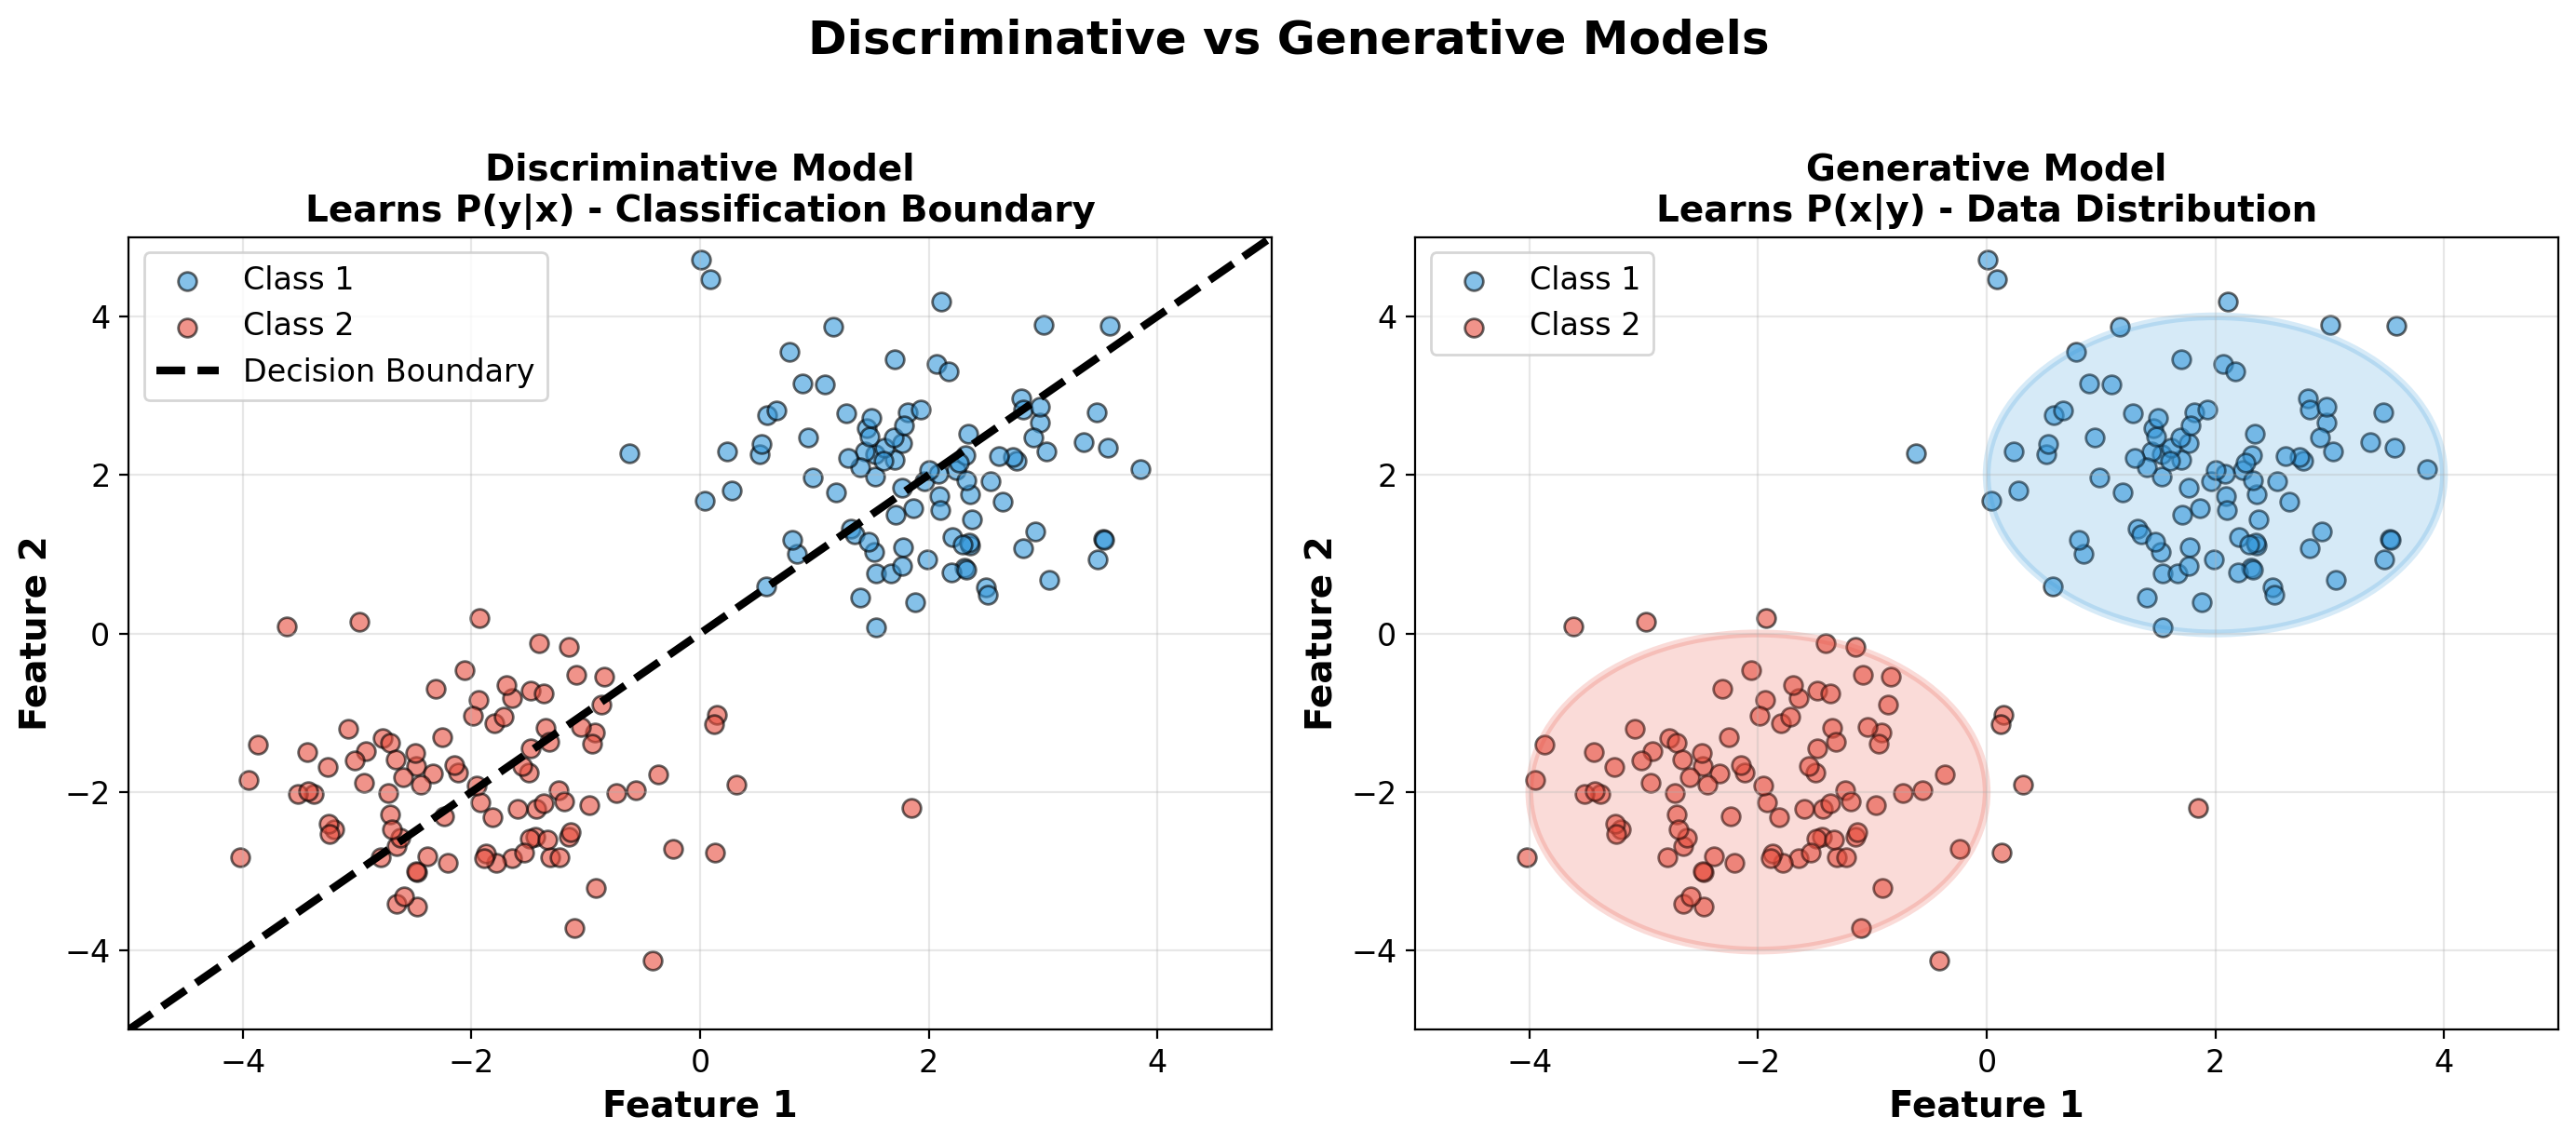
\includegraphics[width=0.85\textwidth]{../figures/generative_vs_discriminative.png}
\end{center}

\textbf{Key Difference:} Discriminative models classify, generative models create
\end{frame}

\begin{frame}{Types of Generative Models}
\textbf{We'll Cover Two Main Approaches:}

\begin{columns}
\column{0.48\textwidth}
\textbf{Variational Autoencoders (VAE):}
\begin{itemize}
\item Learn compressed representation
\item Probabilistic approach
\item Stable training
\item Slightly blurry outputs
\end{itemize}

\column{0.48\textwidth}
\textbf{Generative Adversarial Networks (GAN):}
\begin{itemize}
\item Two networks compete
\item Adversarial training
\item Sharp, realistic outputs
\item Can be tricky to train
\end{itemize}
\end{columns}

\vspace{0.3cm}
\textbf{Both approaches:} Learn from data → Generate new samples
\end{frame}

\section{Autoencoders: The Foundation}

\begin{frame}{What is an Autoencoder?}
\begin{alertblock}{Simple Idea}
Compress an image into a small code, then reconstruct it back. Like a smart ZIP file that learns compression!
\end{alertblock}

\textbf{Two Parts:}
\begin{itemize}
\item \textbf{Encoder:} Compress image → Small code (like squeezing a sponge)
\item \textbf{Decoder:} Small code → Reconstructed image (release the sponge)
\end{itemize}

\textbf{Why Useful?}
\begin{itemize}
\item Forces network to learn important features
\item Throws away noise and details
\item Creates useful compressed representation
\end{itemize}
\end{frame}

\begin{frame}{Autoencoder Architecture}
\begin{center}
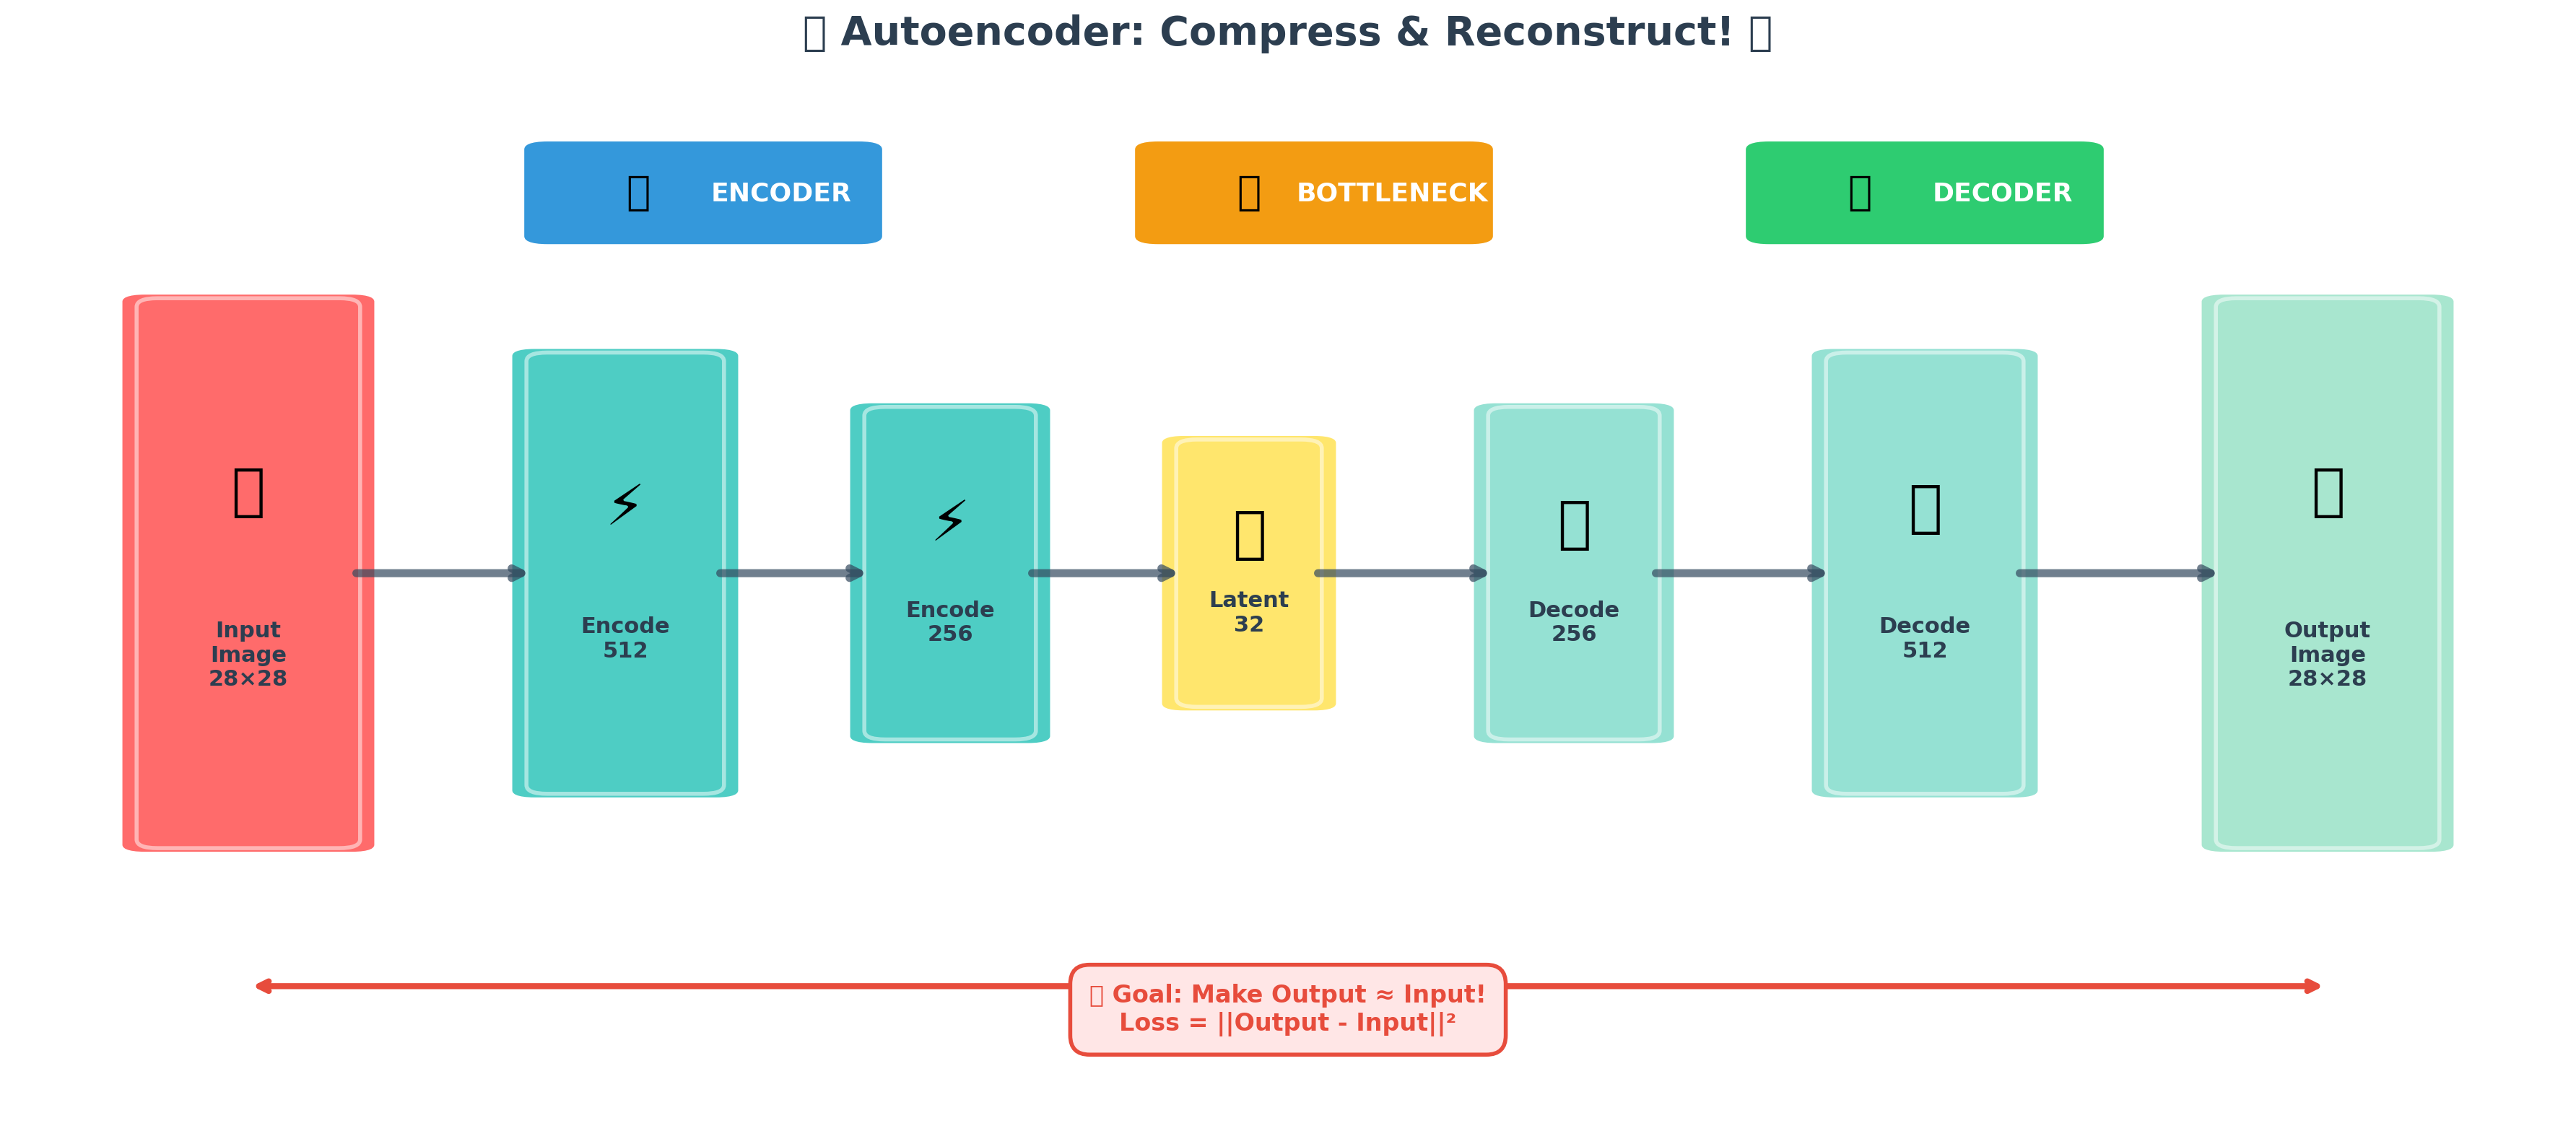
\includegraphics[width=0.75\textwidth]{../figures/autoencoder_architecture.png}
\end{center}

\textbf{Goal:} Make output look like input (minimize reconstruction error)
\end{frame}

\begin{frame}{The Latent Space}
\begin{alertblock}{What is Latent Space?}
The "compressed code" in the middle where similar images are close together. Think of it as a map of all possible images!
\end{alertblock}

\textbf{Analogy:}
\begin{itemize}
\item Full image = Street address (detailed, long)
\item Latent code = GPS coordinates (compact, essential info)
\item Nearby coordinates = Similar locations
\end{itemize}
\end{frame}

\begin{frame}{Latent Space Visualization}
\begin{center}
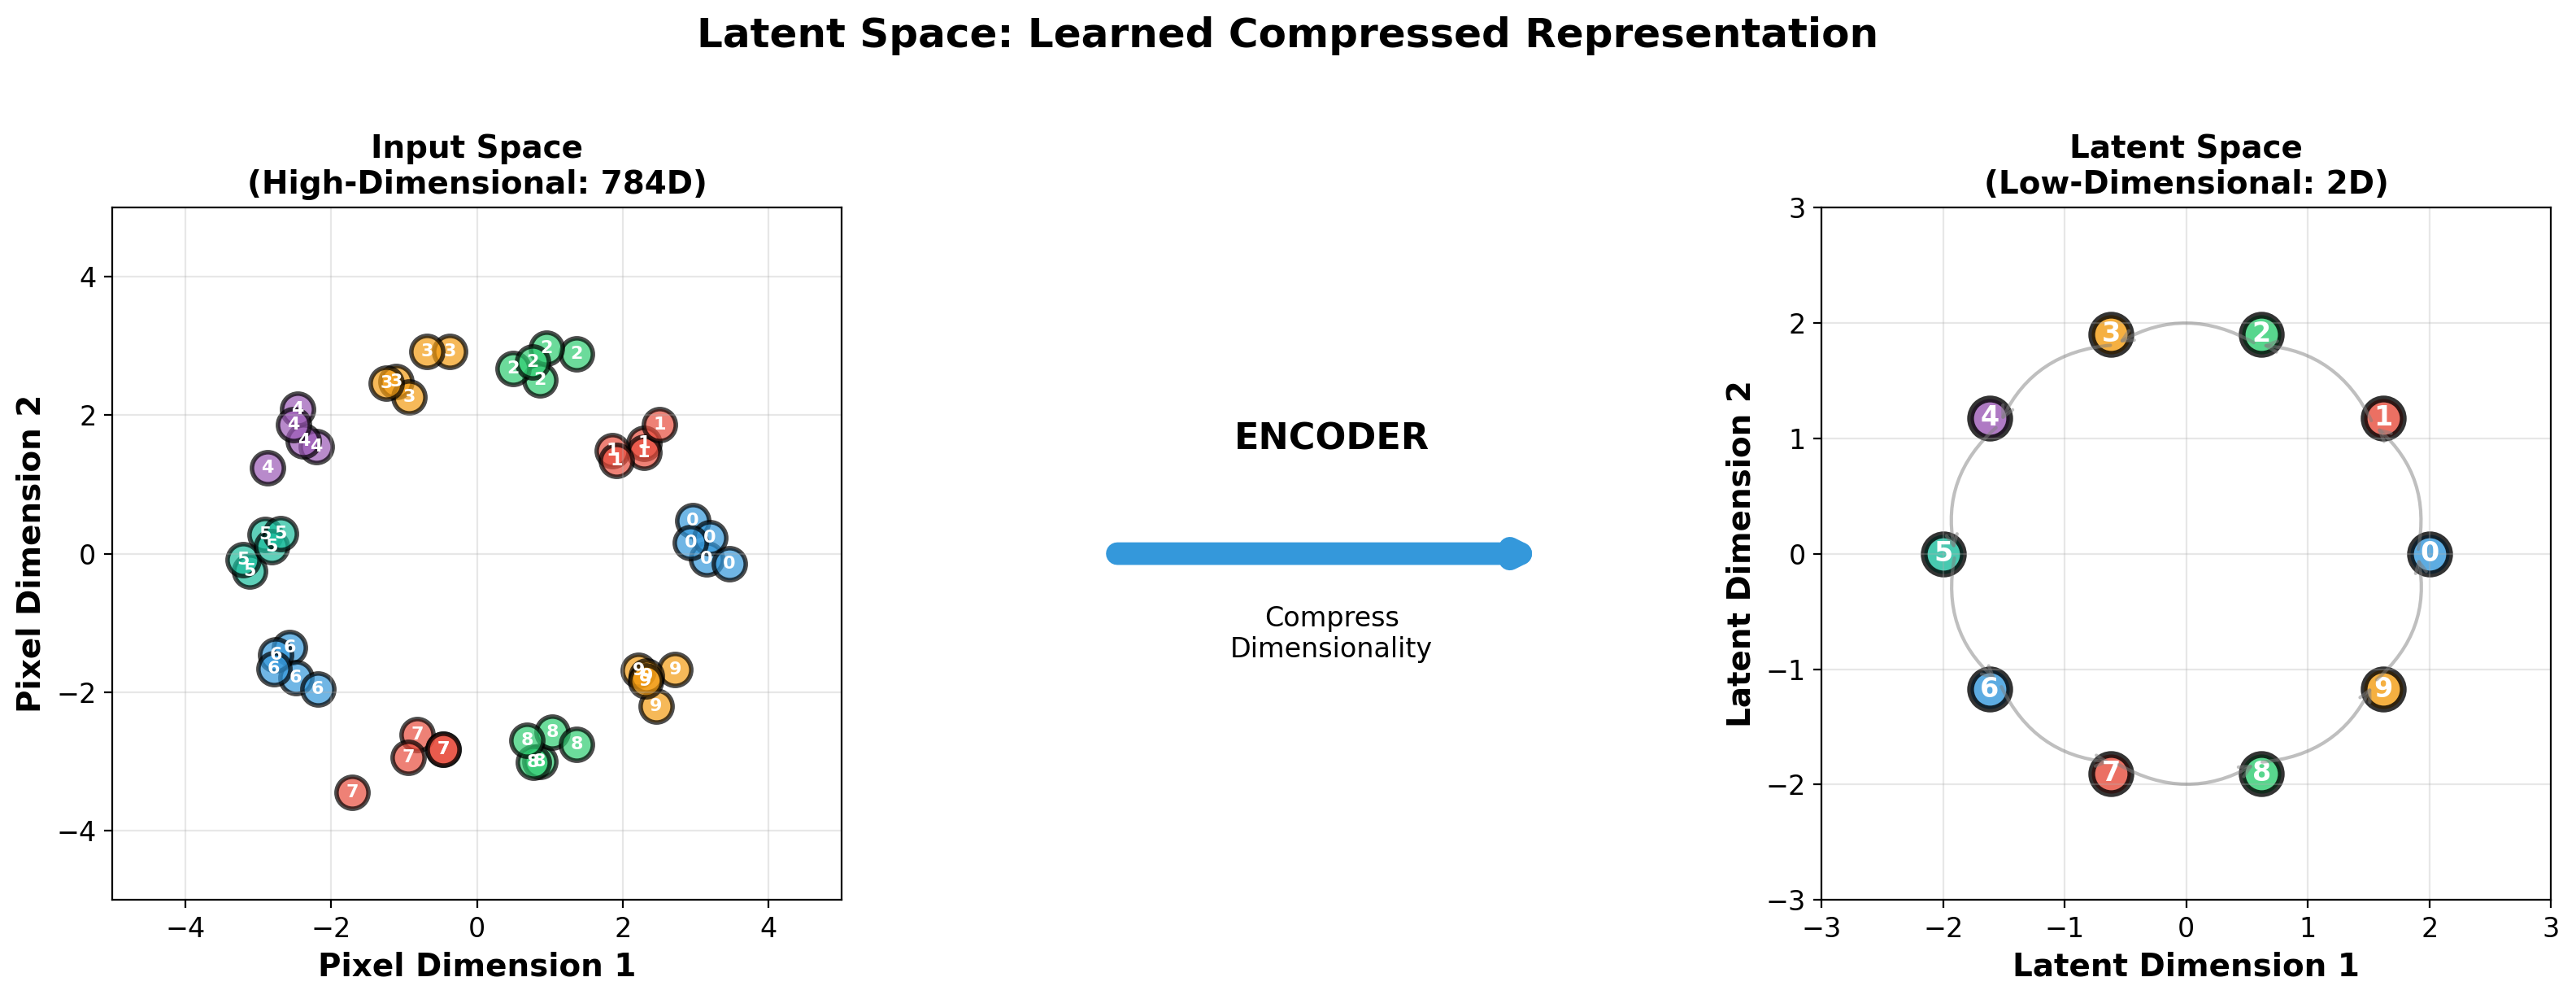
\includegraphics[width=0.9\textwidth]{../figures/latent_space_concept.png}
\end{center}

Compression from 784 dimensions (28×28) to just 2 dimensions
\end{frame}

\begin{frame}{Problem with Basic Autoencoders}
\textbf{Issue:} Can't generate NEW images easily
\begin{itemize}
\item Learns to compress and reconstruct
\item Latent space has "gaps" and irregularities
\item Random sampling gives bad results
\end{itemize}

\textbf{Solution:} Make latent space smooth and continuous → \textbf{Variational Autoencoder (VAE)}
\end{frame}

\section{Variational Autoencoders (VAE)}

\begin{frame}{What Makes VAE Different?}
\begin{alertblock}{Key Insight}
Instead of encoding to a single point, encode to a probability distribution. This creates a smooth, continuous latent space perfect for generation!
\end{alertblock}

\textbf{Regular Autoencoder:}
\begin{itemize}
\item Image → Single code (one point)
\item Gaps in latent space
\end{itemize}

\textbf{VAE:}
\begin{itemize}
\item Image → Distribution of codes (cloud of points)
\item Smooth, continuous latent space
\item Can sample new codes easily
\end{itemize}
\end{frame}

\begin{frame}{VAE Architecture}
\begin{center}
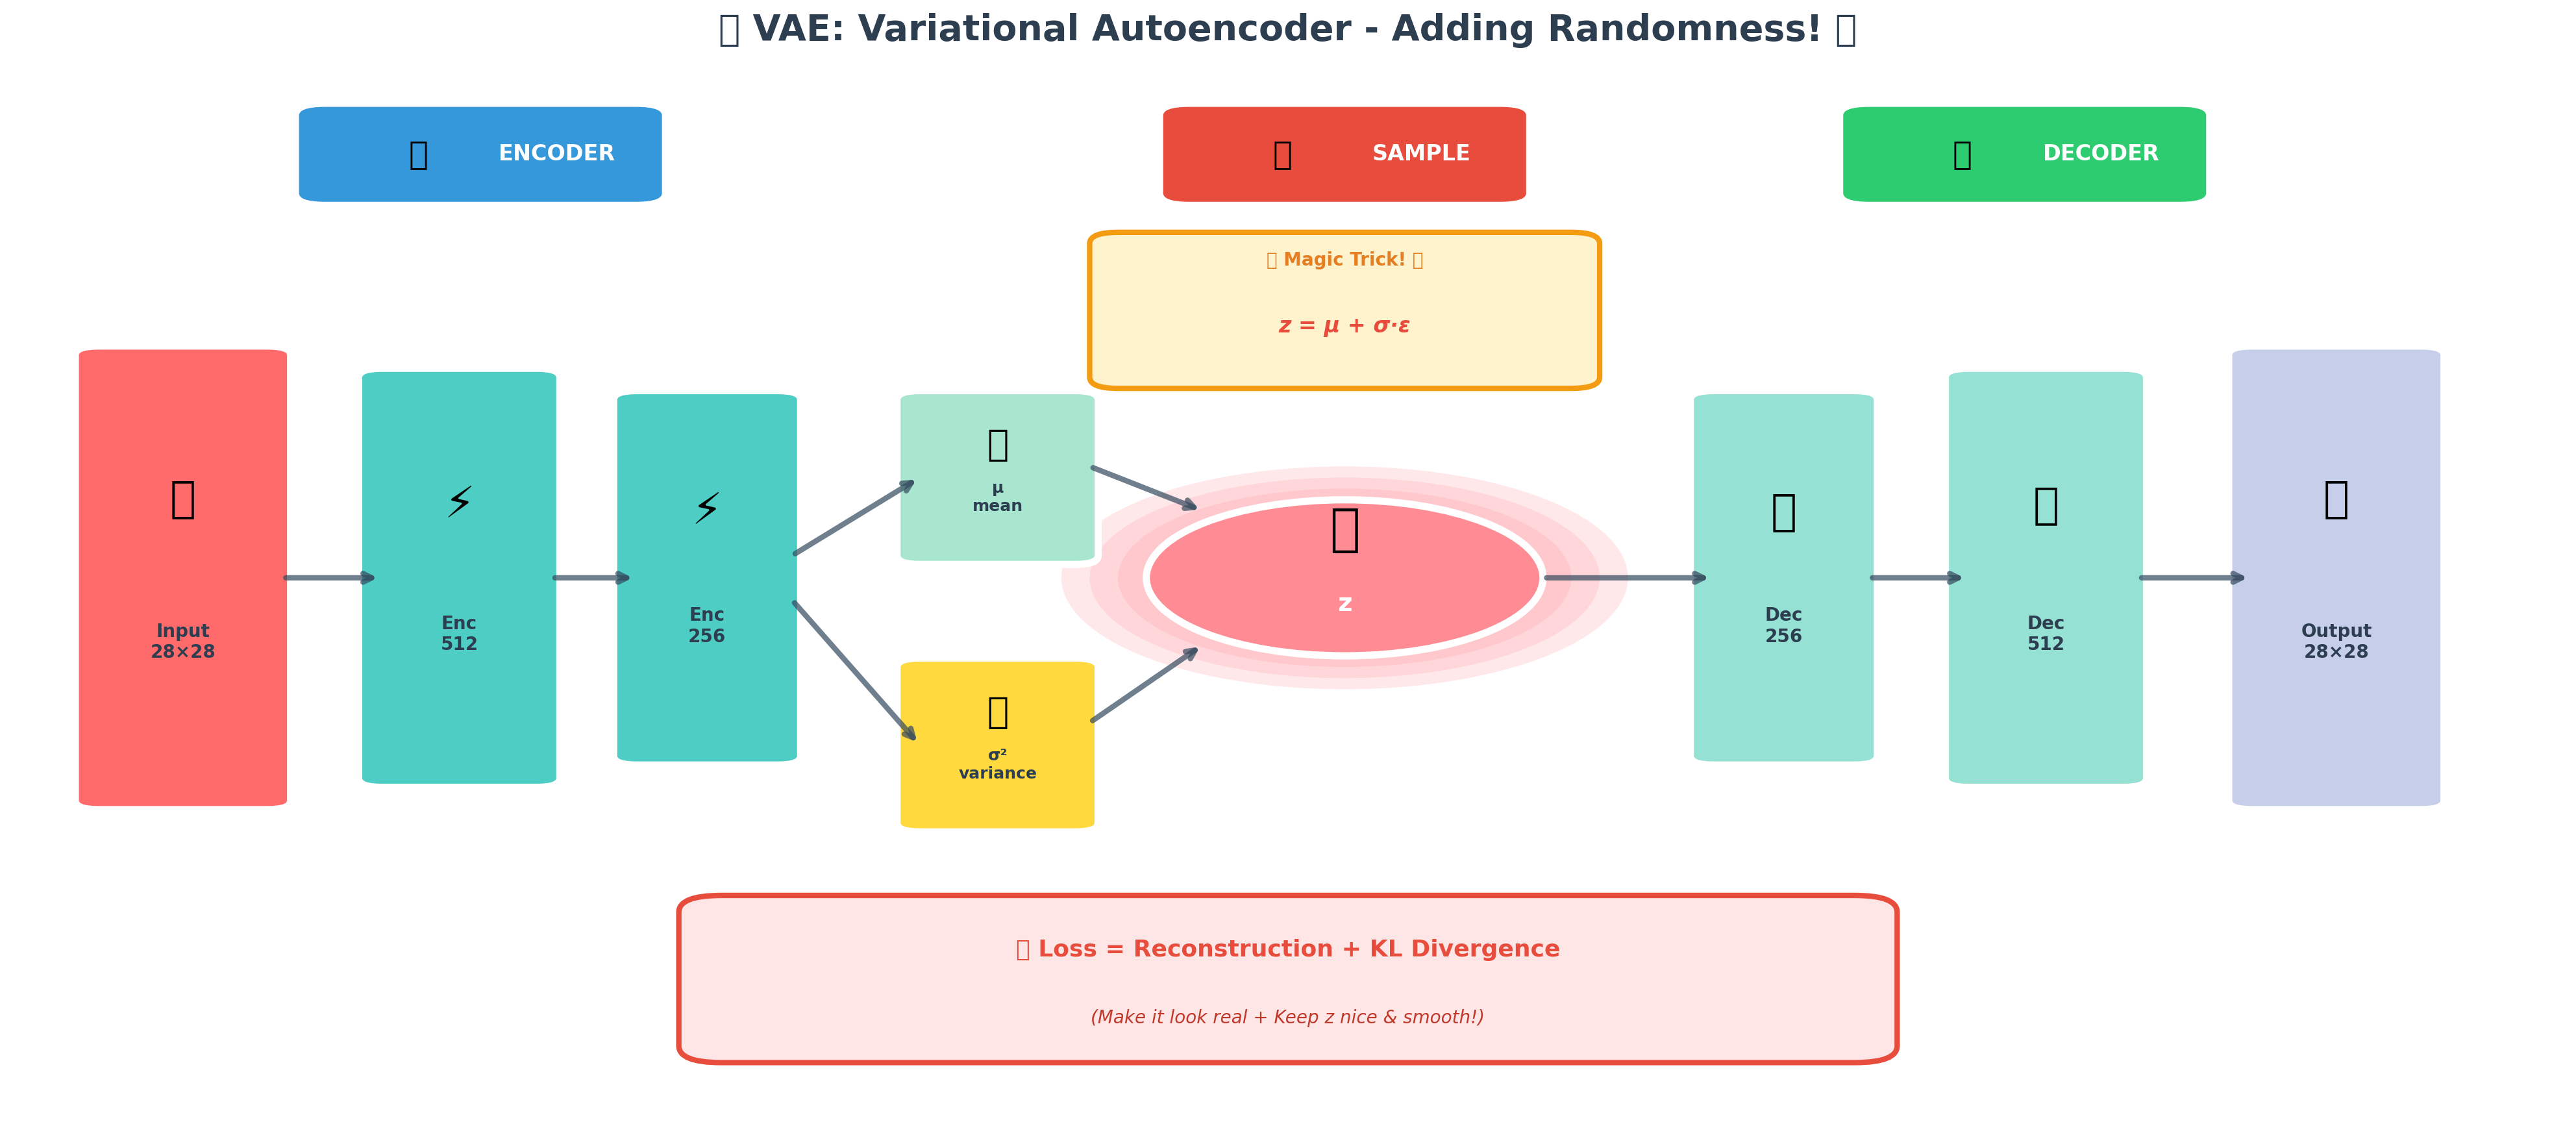
\includegraphics[width=0.7\textwidth]{../figures/vae_architecture.png}
\end{center}

Mean ($\mu$) and variance ($\sigma^2$) instead of single code
\end{frame}

\begin{frame}{How VAE Encoding Works}
\textbf{Step-by-Step:}
\begin{enumerate}
\item Encoder produces mean ($\mu$) and variance ($\sigma^2$)
\item Sample code: $z = \mu + \sigma \cdot \epsilon$ where $\epsilon \sim N(0,1)$
\item Decoder reconstructs from sampled code
\end{enumerate}

\textbf{Why This Helps:}
\begin{itemize}
\item Forces smooth latent space
\item Similar images have overlapping distributions
\end{itemize}
\end{frame}

\begin{frame}{VAE Loss Function (Simplified)}
\textbf{Two Goals:}

\textbf{1. Reconstruction:} Output should look like input
\begin{itemize}
\item $\text{Loss}_{\text{recon}} = || \text{input} - \text{output} ||^2$
\end{itemize}

\textbf{2. Regularization:} Keep distributions close to standard normal
\begin{itemize}
\item KL Divergence: Push $\mu$ toward 0, $\sigma$ toward 1
\item Prevents "cheating"
\end{itemize}

\vspace{0.3cm}
\textbf{Total Loss} = Reconstruction + KL Divergence

Balance is key!
\end{frame}

\begin{frame}{VAE Sampling Process}
\begin{center}
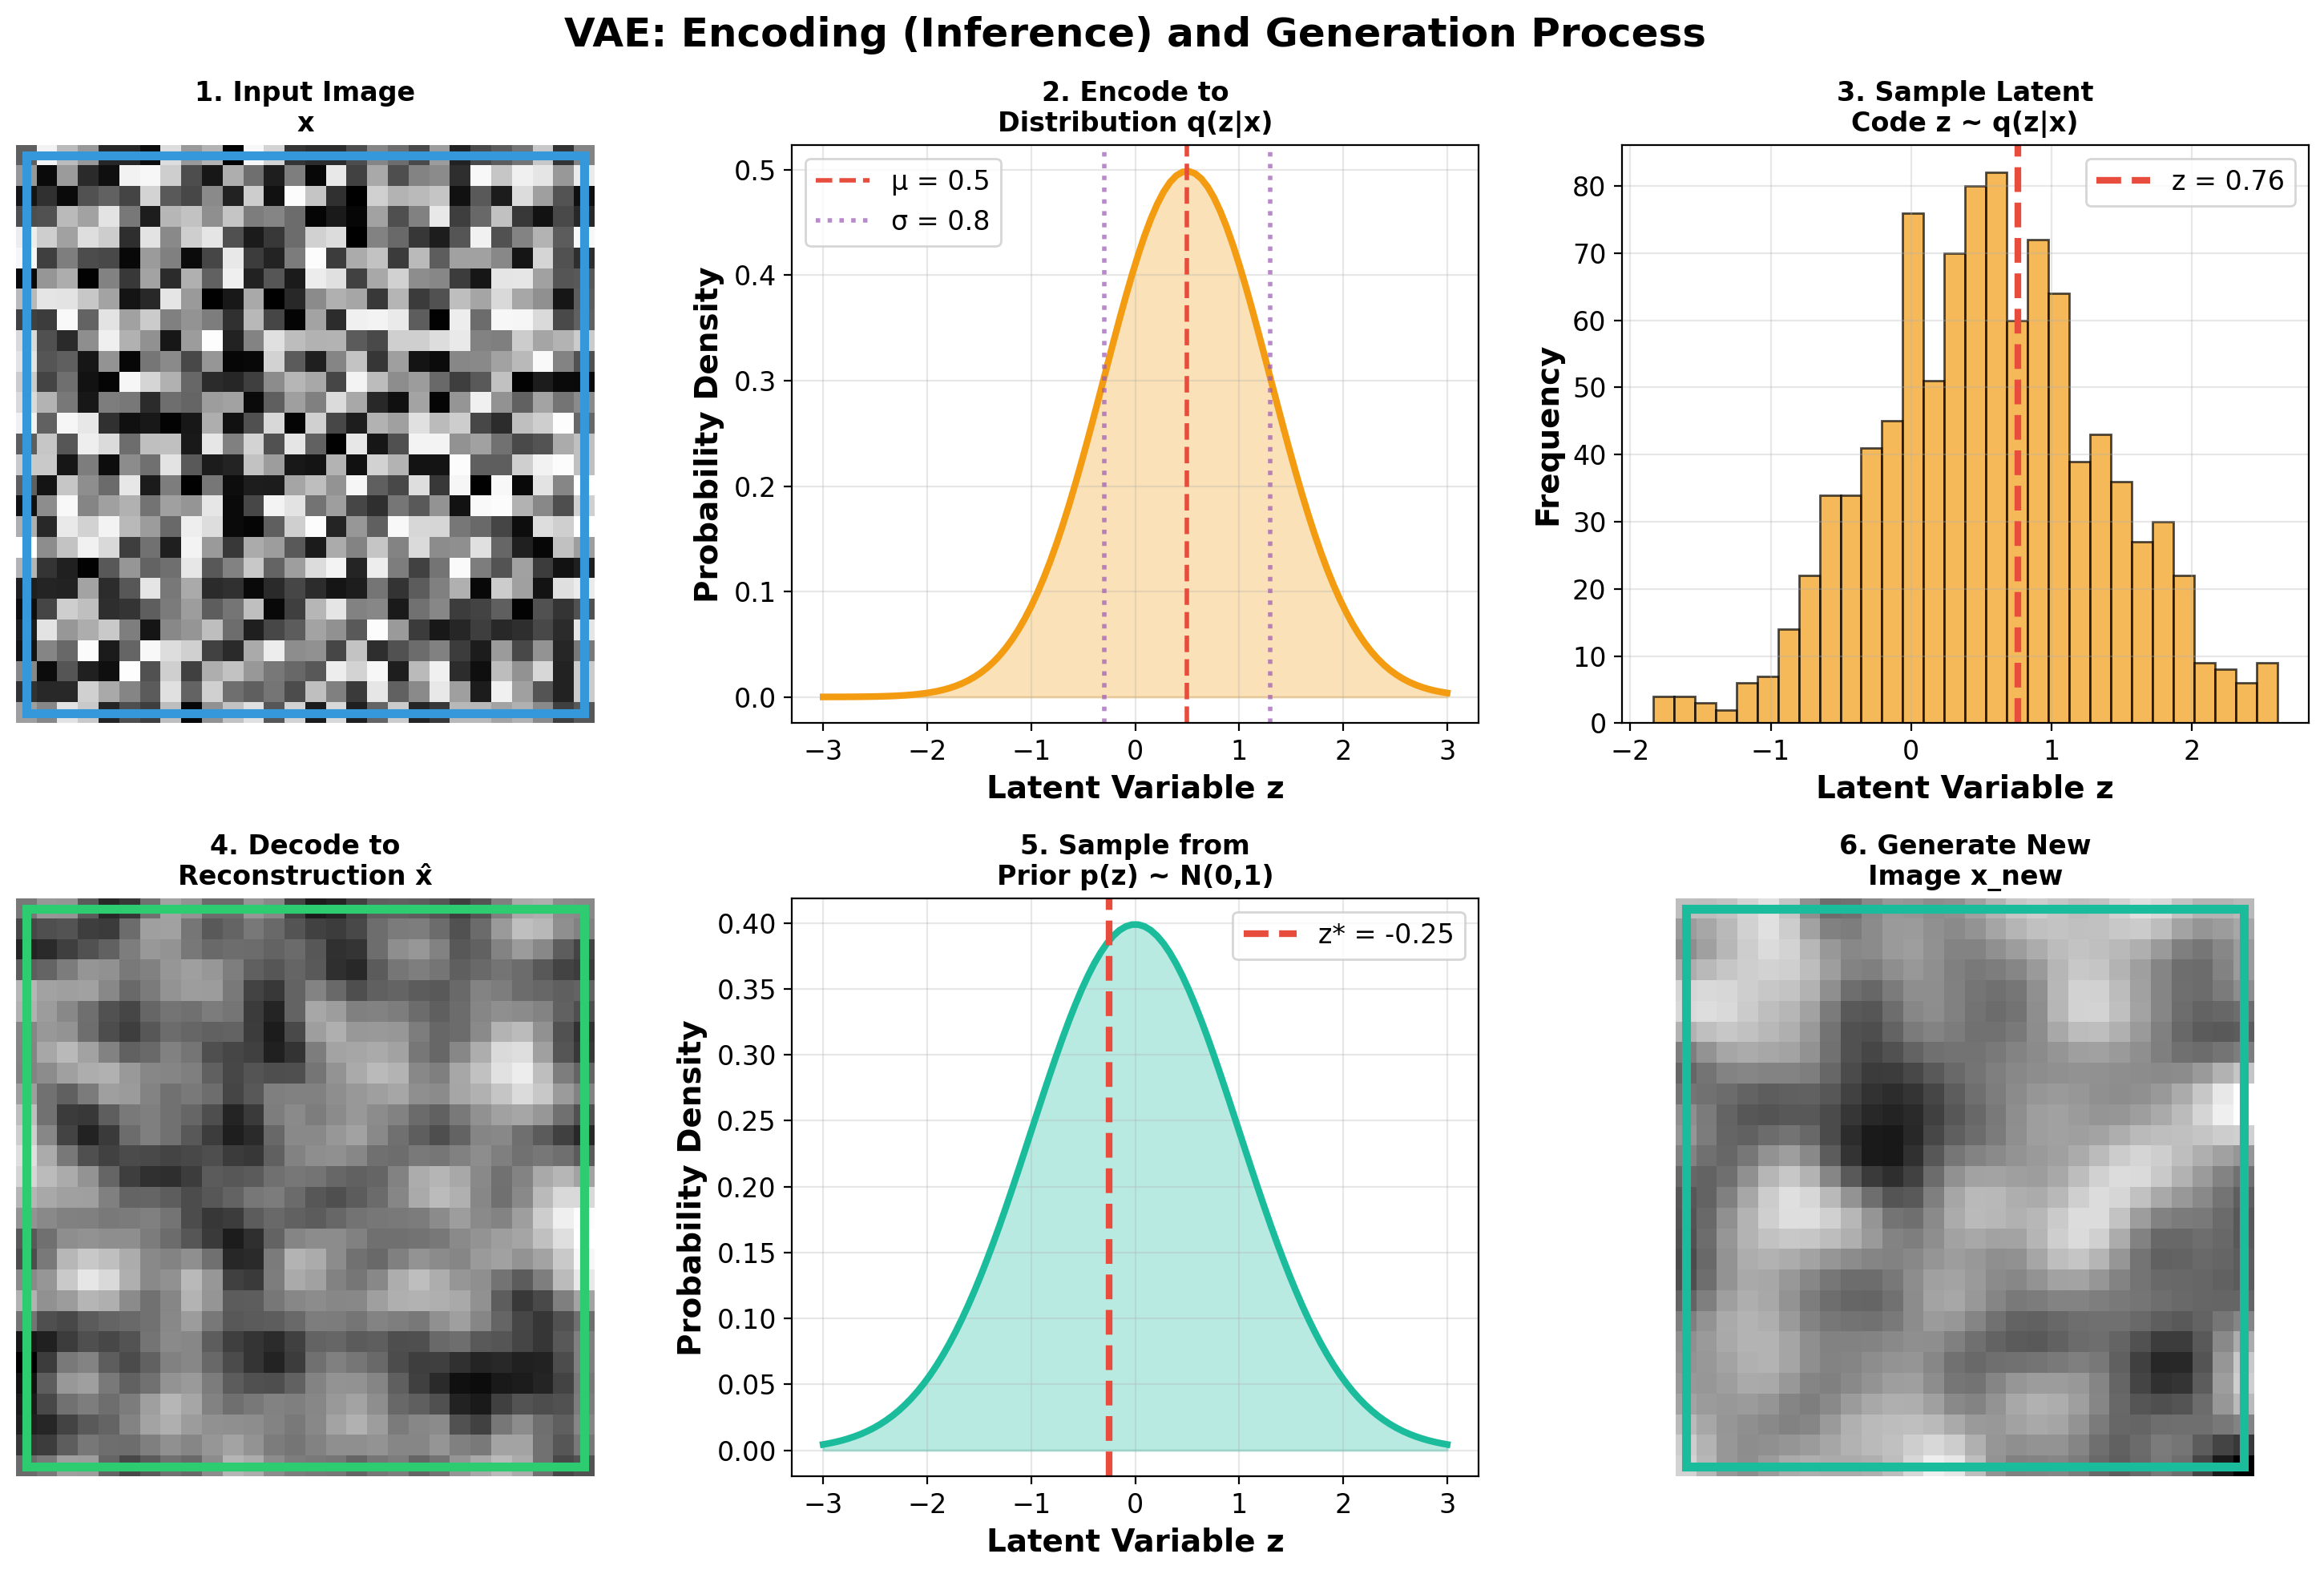
\includegraphics[width=0.65\textwidth]{../figures/vae_sampling_process.png}
\end{center}

Top: Encoding. Bottom: Generation
\end{frame}

\begin{frame}{VAE for Generation}
\textbf{Two Ways to Generate:}

\textbf{1. Reconstruction:}
\begin{itemize}
\item Encode real image
\item Sample from learned distribution
\item Decode to get similar image
\end{itemize}

\textbf{2. Pure Generation:}
\begin{itemize}
\item Sample random code from $N(0,1)$
\item Decode to get completely new image
\item Works because latent space is smooth!
\end{itemize}
\end{frame}

\begin{frame}{VAE Pros and Cons}
\textbf{Advantages:}
\begin{itemize}
\item Stable and easy to train
\item Smooth latent space
\item Principled probabilistic framework
\item Good for interpolation
\end{itemize}

\textbf{Limitations:}
\begin{itemize}
\item Outputs tend to be blurry
\item Less sharp than real images
\item Trade-off between quality and smoothness
\end{itemize}

\textbf{Best for:} Understanding data structure, interpolation, compression
\end{frame}

\section{Generative Adversarial Networks (GAN)}

\begin{frame}{GAN: A Different Approach}
\begin{alertblock}{Core Idea}
Two networks compete: Generator tries to create fake images, Discriminator tries to spot fakes. Competition makes both better!
\end{alertblock}

\textbf{Analogy:} Art Forger vs Art Detective
\begin{itemize}
\item \textbf{Forger (Generator):} Creates fake paintings, improves to fool detective
\item \textbf{Detective (Discriminator):} Learns to spot fakes, gets better over time
\item \textbf{Result:} Forger becomes so good, detective can't tell real from fake!
\end{itemize}
\end{frame}

\begin{frame}{GAN Architecture}
\begin{center}
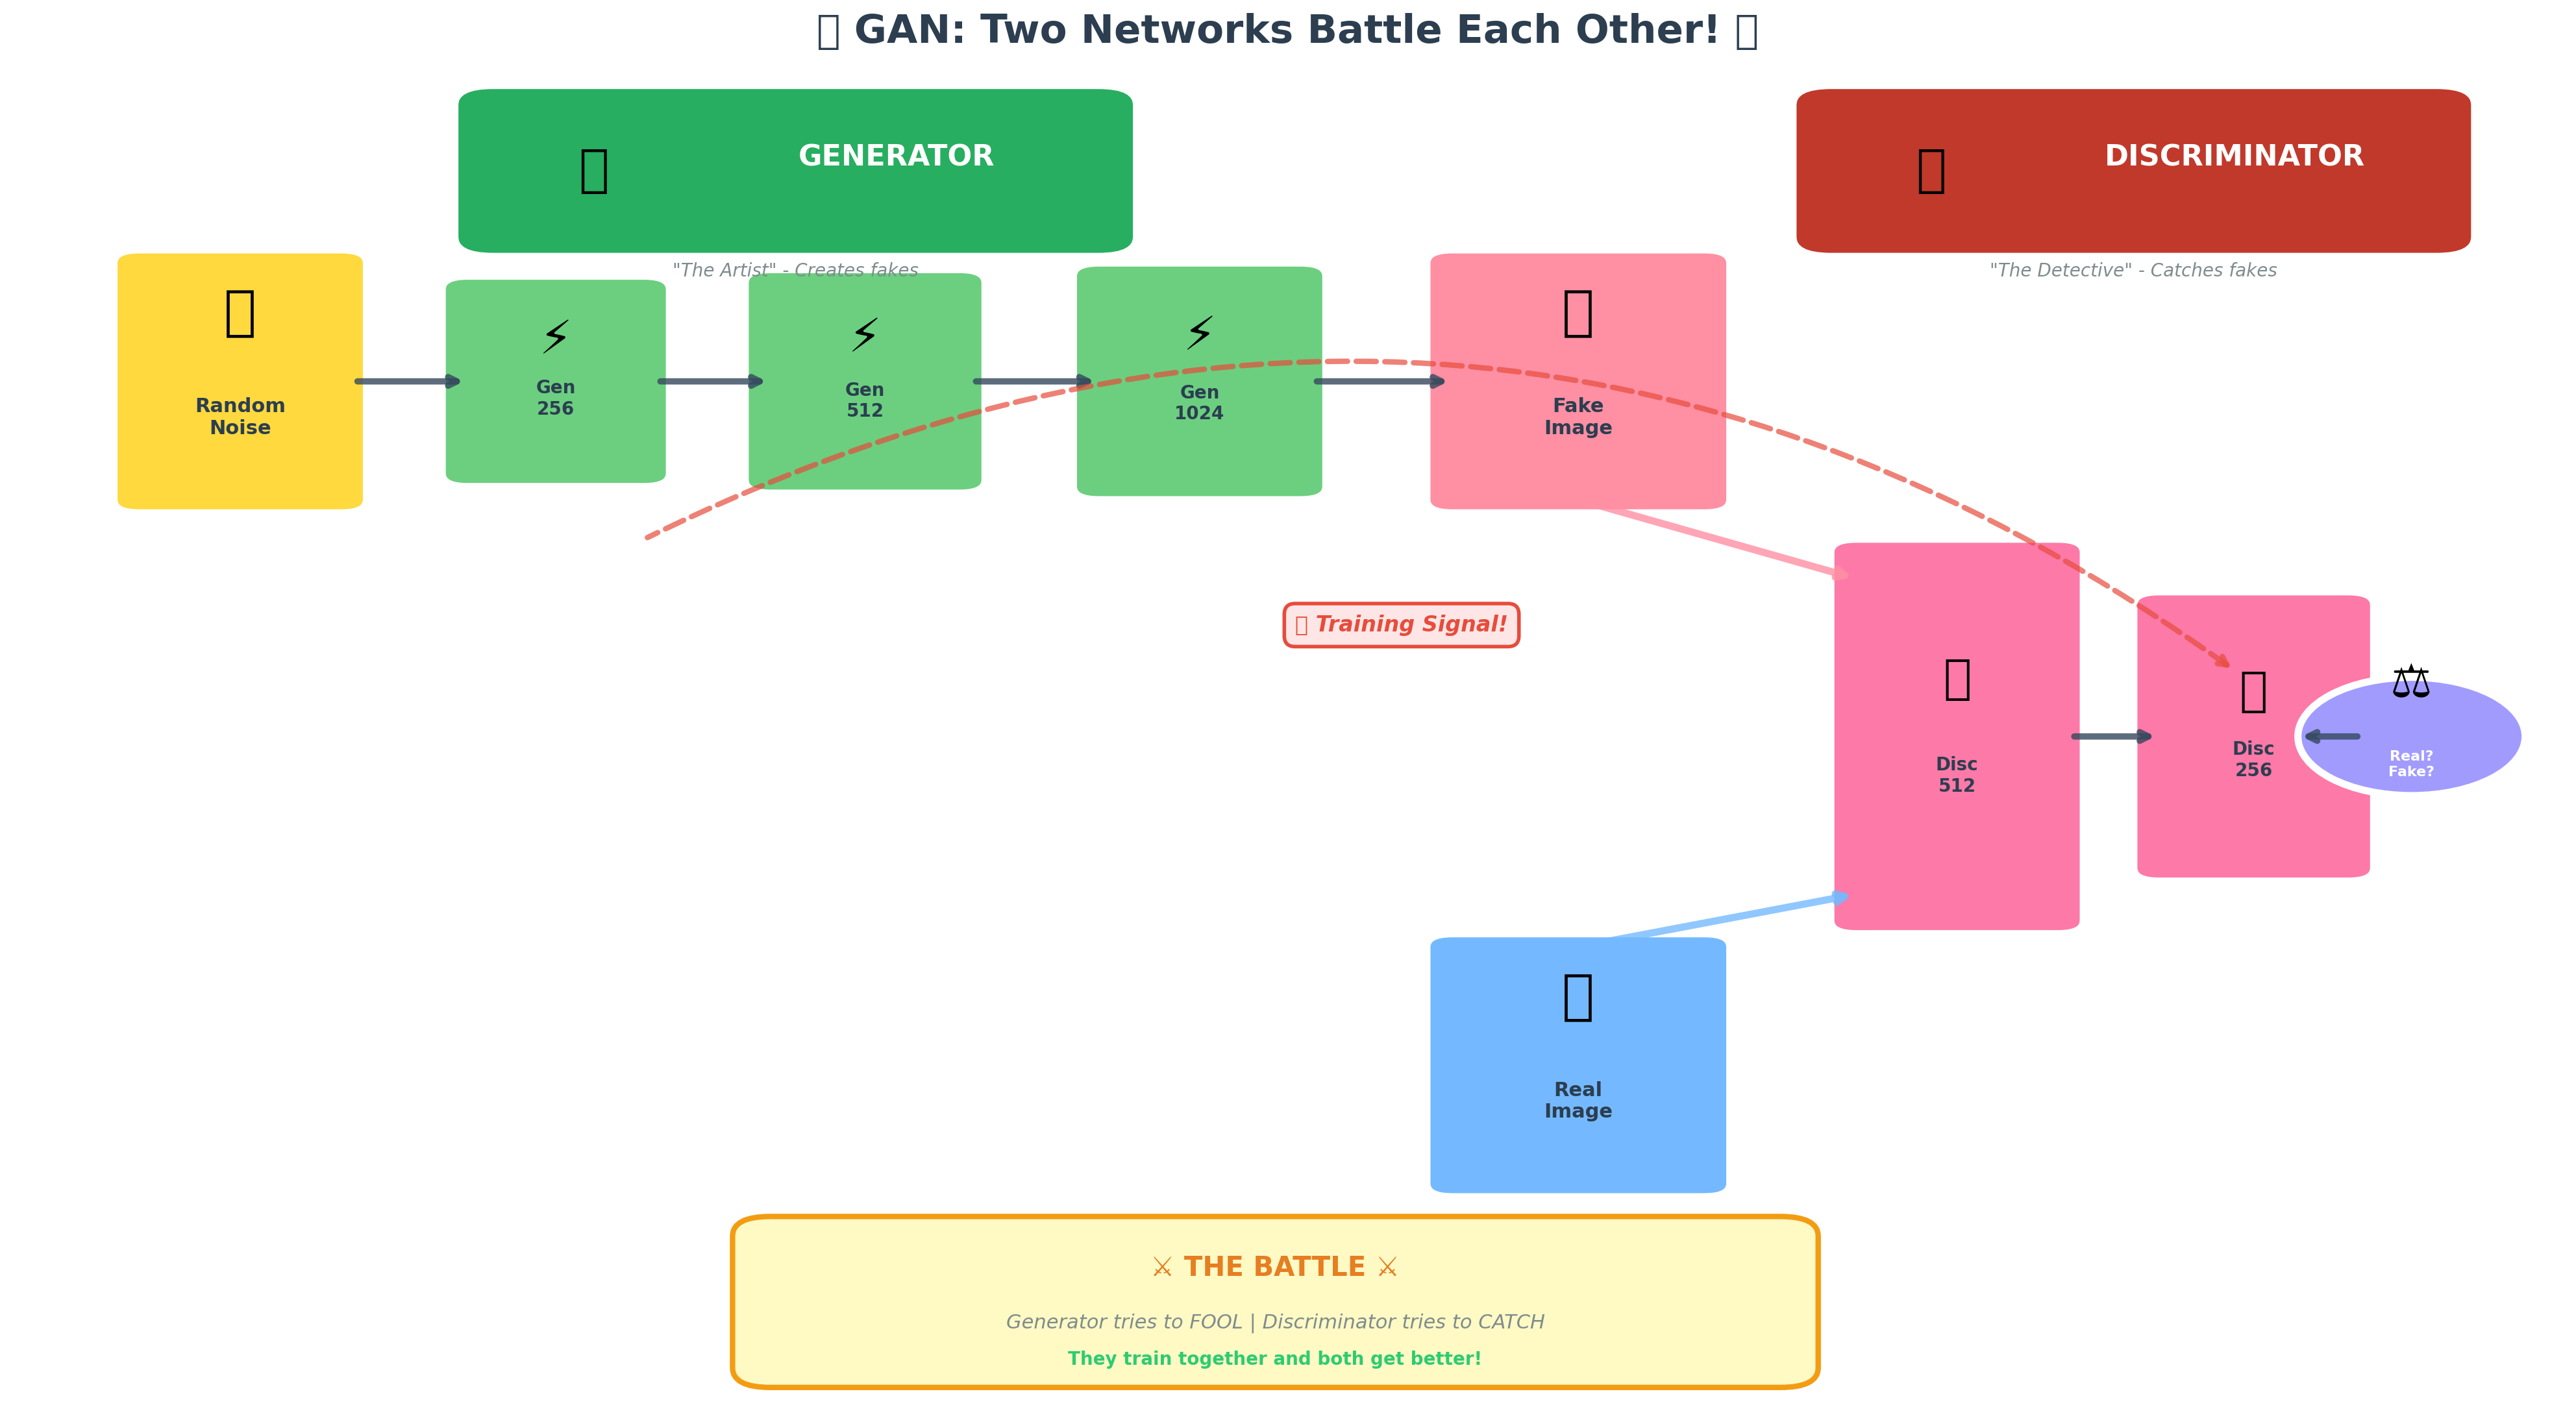
\includegraphics[width=0.7\textwidth]{../figures/gan_architecture.png}
\end{center}

Two networks trained simultaneously in competition
\end{frame}

\begin{frame}{How GAN Training Works}
\textbf{Training Loop:}

\textbf{1. Train Discriminator:}
\begin{itemize}
\item Show real images → Label "real" (1)
\item Show fake images from generator → Label "fake" (0)
\item Update D to get better at classification
\end{itemize}

\textbf{2. Train Generator:}
\begin{itemize}
\item Generate fake images
\item Try to fool discriminator
\item Update G based on discriminator's response
\end{itemize}

\textbf{Repeat:} Alternate between training D and G
\end{frame}

\begin{frame}{GAN as a Game}
\begin{center}
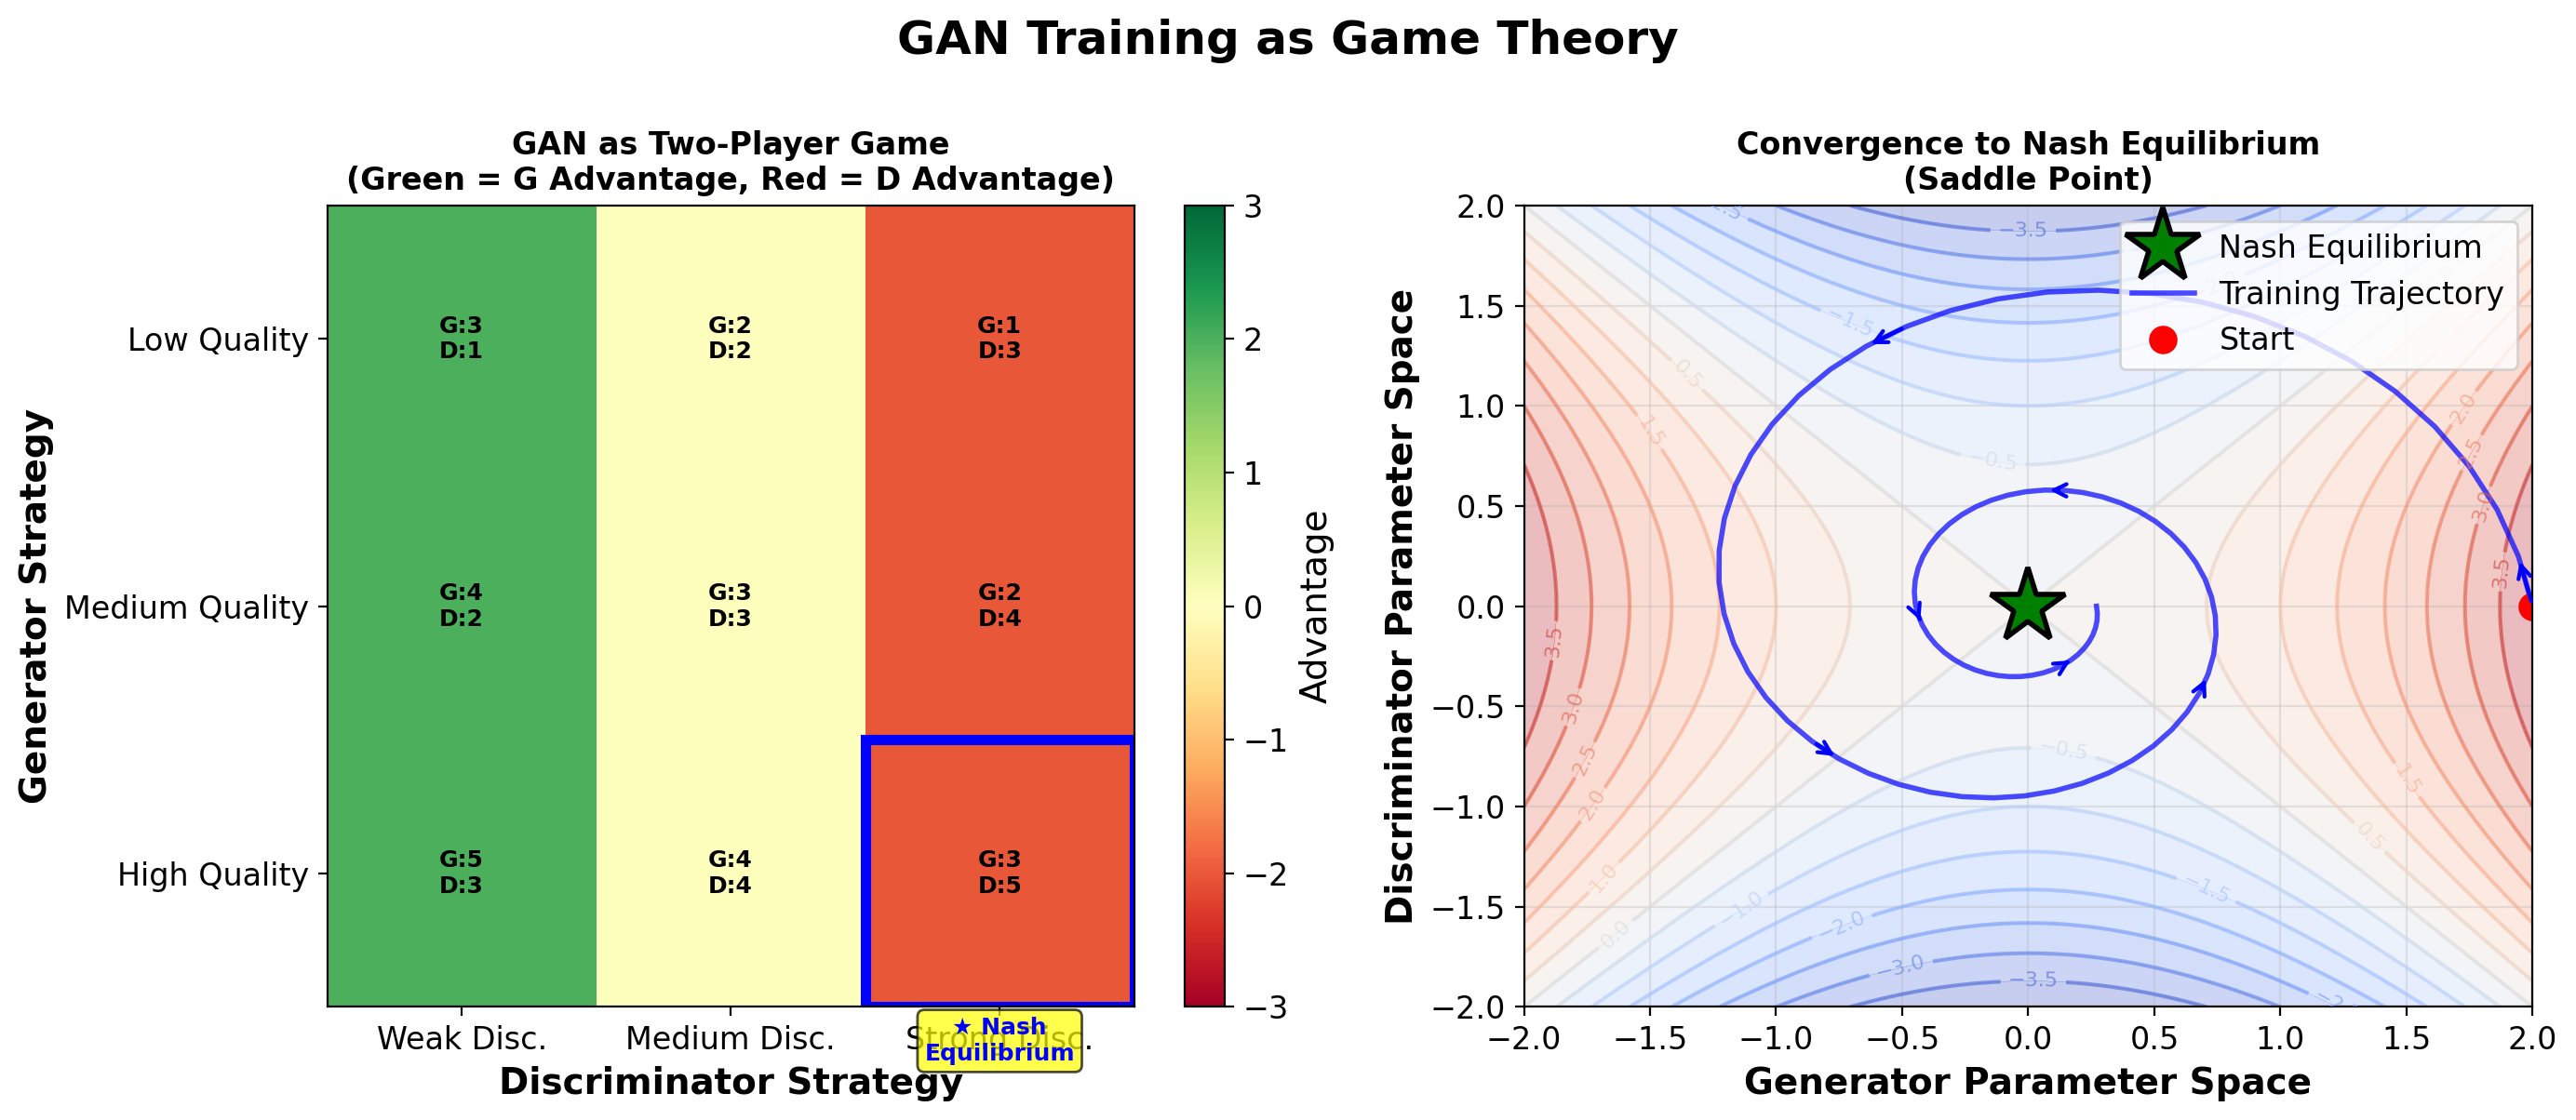
\includegraphics[width=0.85\textwidth]{../figures/gan_game_theory.png}
\end{center}

\textbf{Goal:} Reach Nash equilibrium where neither can improve
\end{frame}

\begin{frame}{GAN Training Dynamics}
\begin{center}
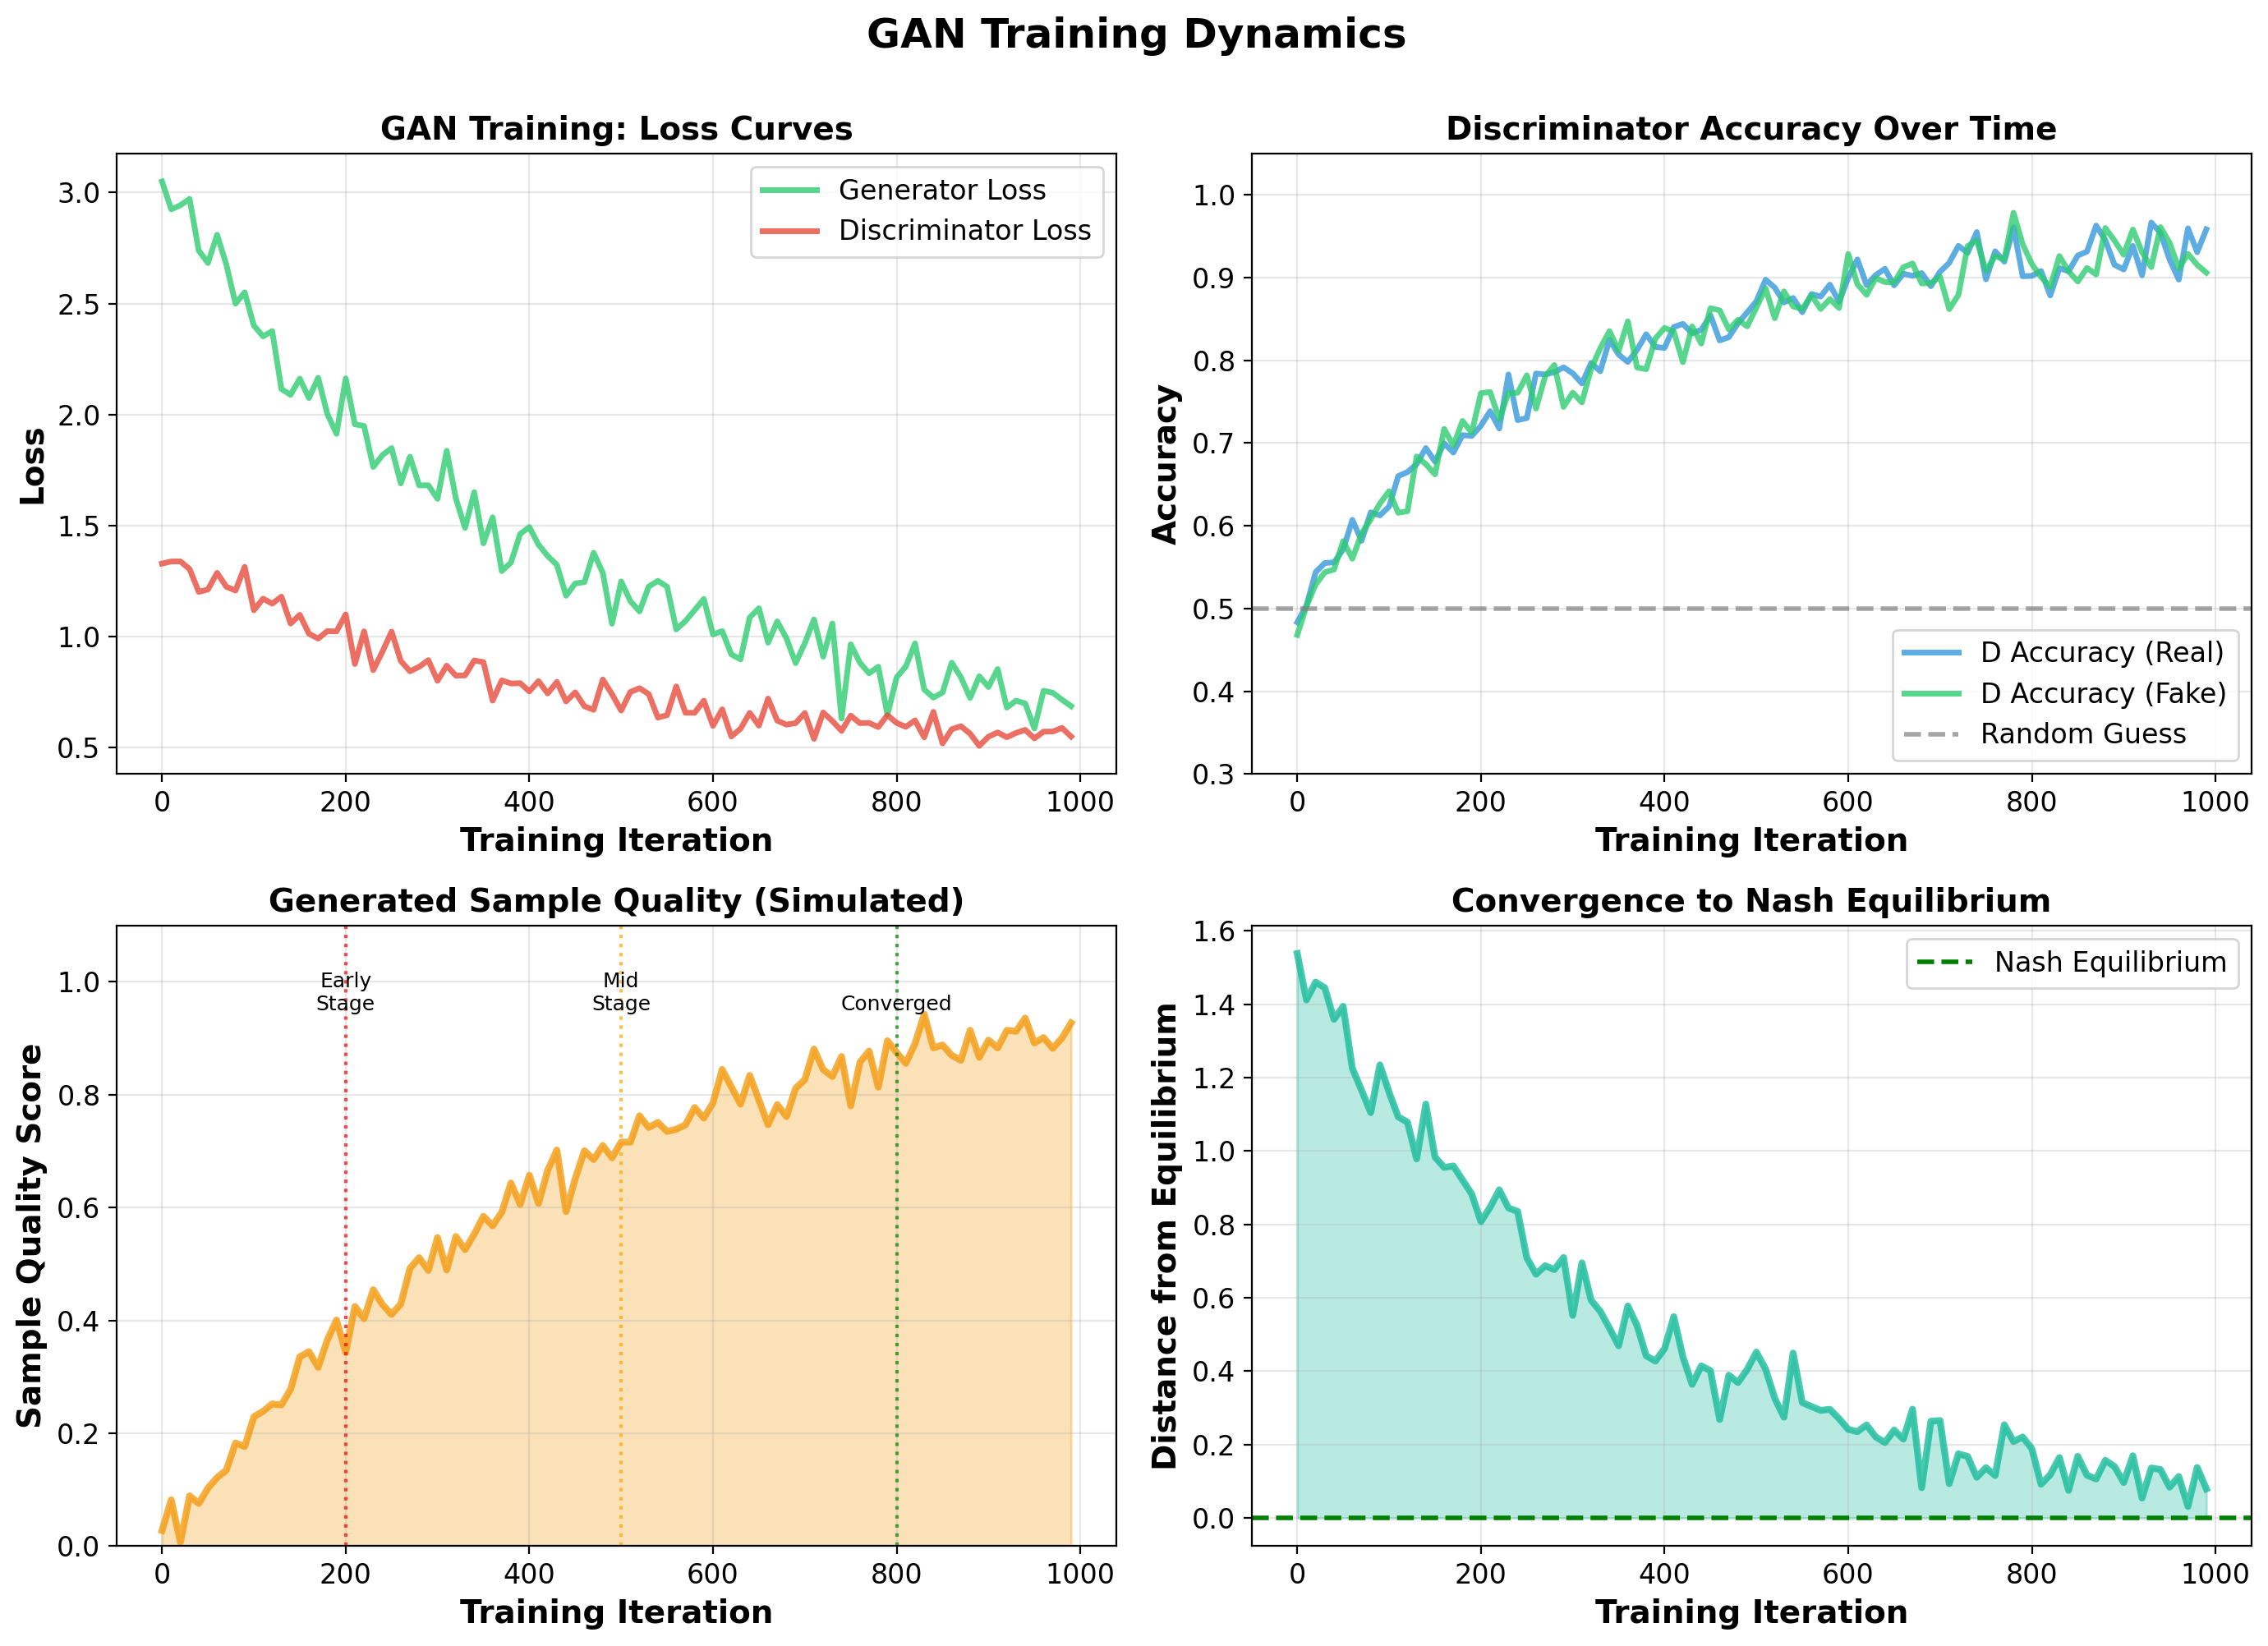
\includegraphics[width=0.62\textwidth]{../figures/gan_training_dynamics.png}
\end{center}
\end{frame}

\begin{frame}{GAN Challenges - Part 1}
\textbf{1. Training Instability:}
\begin{itemize}
\item Hard to balance G and D
\item One can dominate the other
\item Requires careful tuning
\end{itemize}

\textbf{2. Mode Collapse:}
\begin{itemize}
\item Generator produces limited variety
\item Ignores some modes of data
\item Repetitive outputs
\end{itemize}
\end{frame}

\begin{frame}{Mode Collapse Problem}
\begin{center}
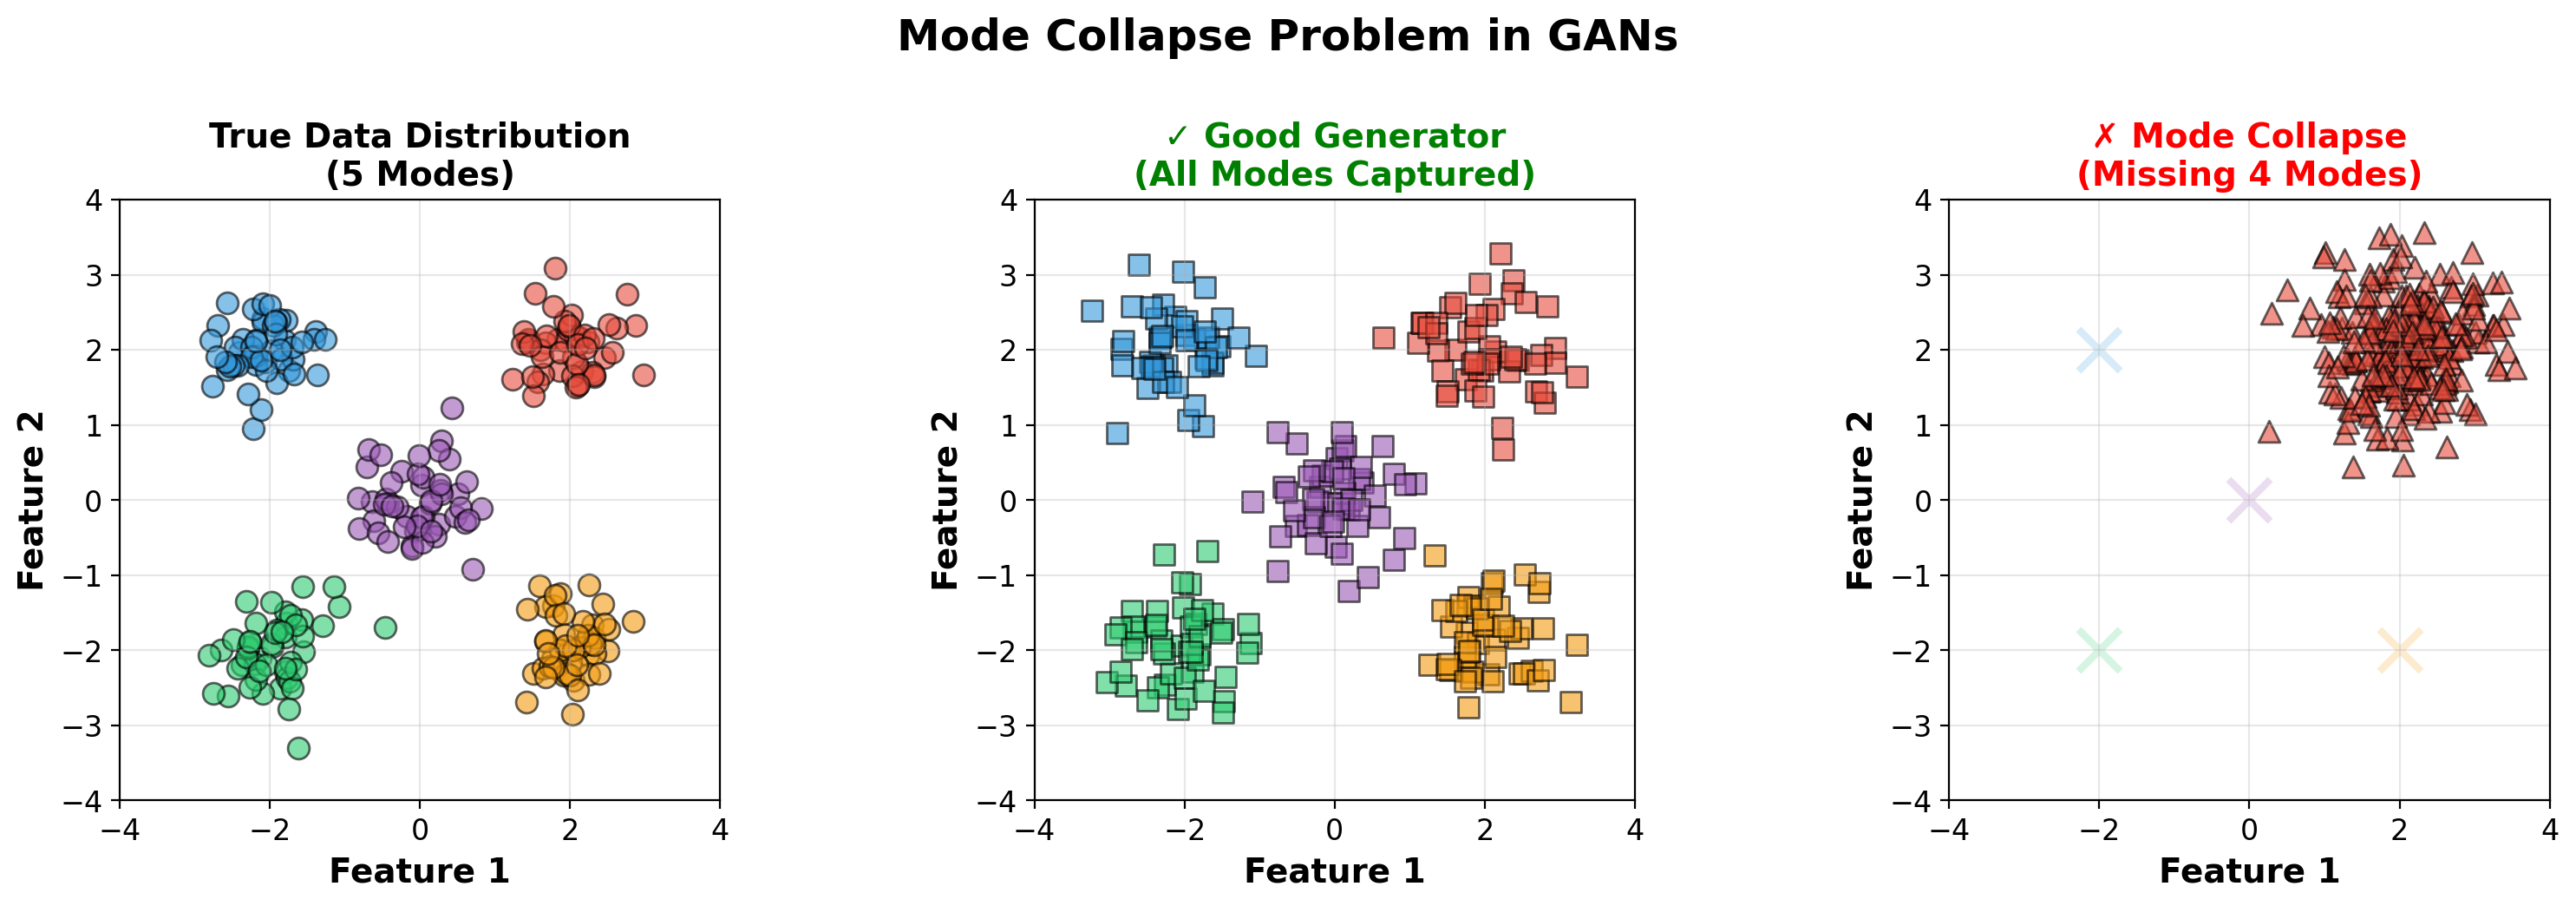
\includegraphics[width=0.85\textwidth]{../figures/mode_collapse.png}
\end{center}

Generator fails to capture full diversity of data
\end{frame}

\begin{frame}{GAN Challenges - Part 2}
\textbf{3. Vanishing Gradients:}
\begin{itemize}
\item If D is too good, G gets no useful feedback
\item Learning stops
\item Need to carefully balance
\end{itemize}

\textbf{4. Evaluation Difficulty:}
\begin{itemize}
\item No single metric for quality
\item Visual inspection needed
\item Inception Score and FID commonly used
\end{itemize}
\end{frame}

\begin{frame}{GAN Training Tips}
\textbf{Best Practices:}
\begin{itemize}
\item Use batch normalization
\item Add label smoothing (0.9 not 1.0)
\item Add noise to discriminator inputs
\item Use Adam optimizer, low learning rate
\item Monitor both losses
\end{itemize}

\textbf{Key Insight:} Balance is everything!
\end{frame}

\begin{frame}{GAN Pros and Cons}
\textbf{Advantages:}
\begin{itemize}
\item Sharp, realistic outputs
\item High quality generations
\item No explicit likelihood needed
\item Creative applications
\end{itemize}

\textbf{Limitations:}
\begin{itemize}
\item Difficult to train
\item Mode collapse issues
\item No probabilistic interpretation
\item Requires careful tuning
\end{itemize}

\textbf{Best for:} High-quality image generation, realistic samples
\end{frame}

\section{VAE vs GAN Comparison}

\begin{frame}{VAE vs GAN: Side by Side}
\begin{center}
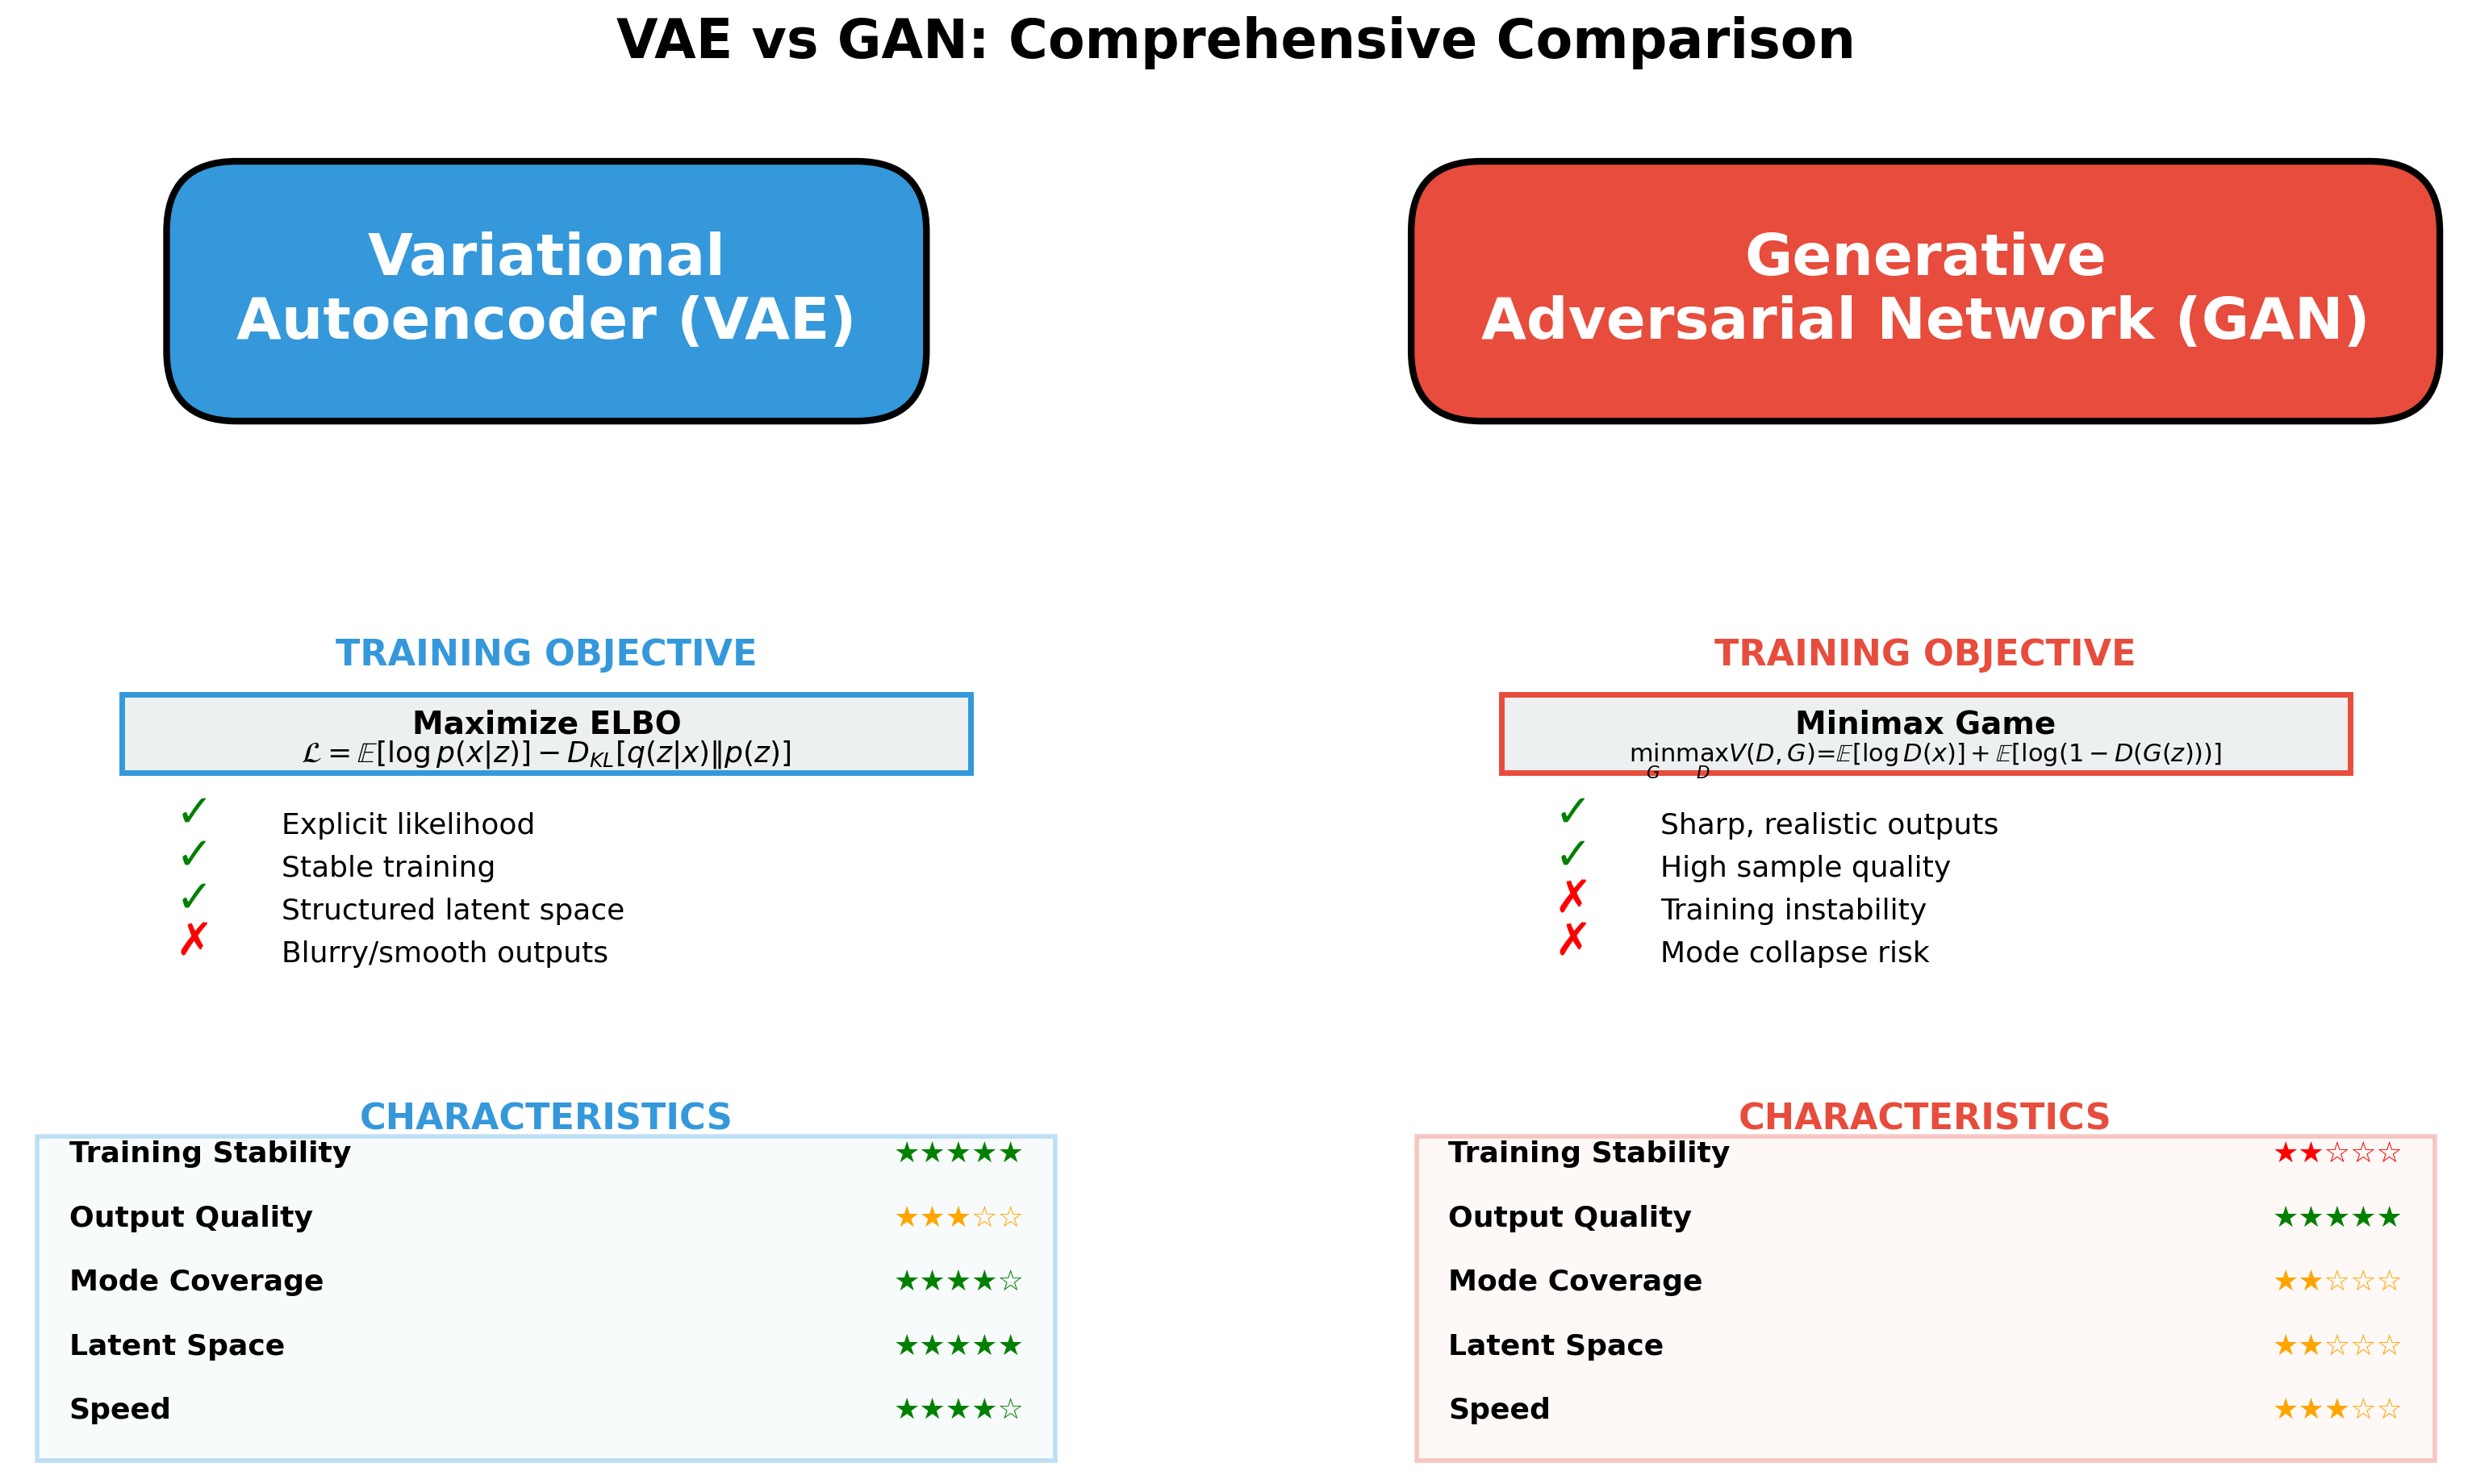
\includegraphics[width=0.8\textwidth]{../figures/vae_vs_gan.png}
\end{center}
\end{frame}

\begin{frame}{When to Use Which?}
\textbf{Choose VAE when:}
\begin{itemize}
\item Need stable training
\item Want smooth latent space
\item Interpolation is important
\item Understanding data structure is goal
\item Probabilistic framework needed
\end{itemize}

\textbf{Choose GAN when:}
\begin{itemize}
\item Image quality is critical
\item Have time for tuning
\item Realistic samples needed
\item Don't need latent space interpretation
\end{itemize}
\end{frame}

\section{Applications}

\begin{frame}{Generation Examples}
\begin{center}
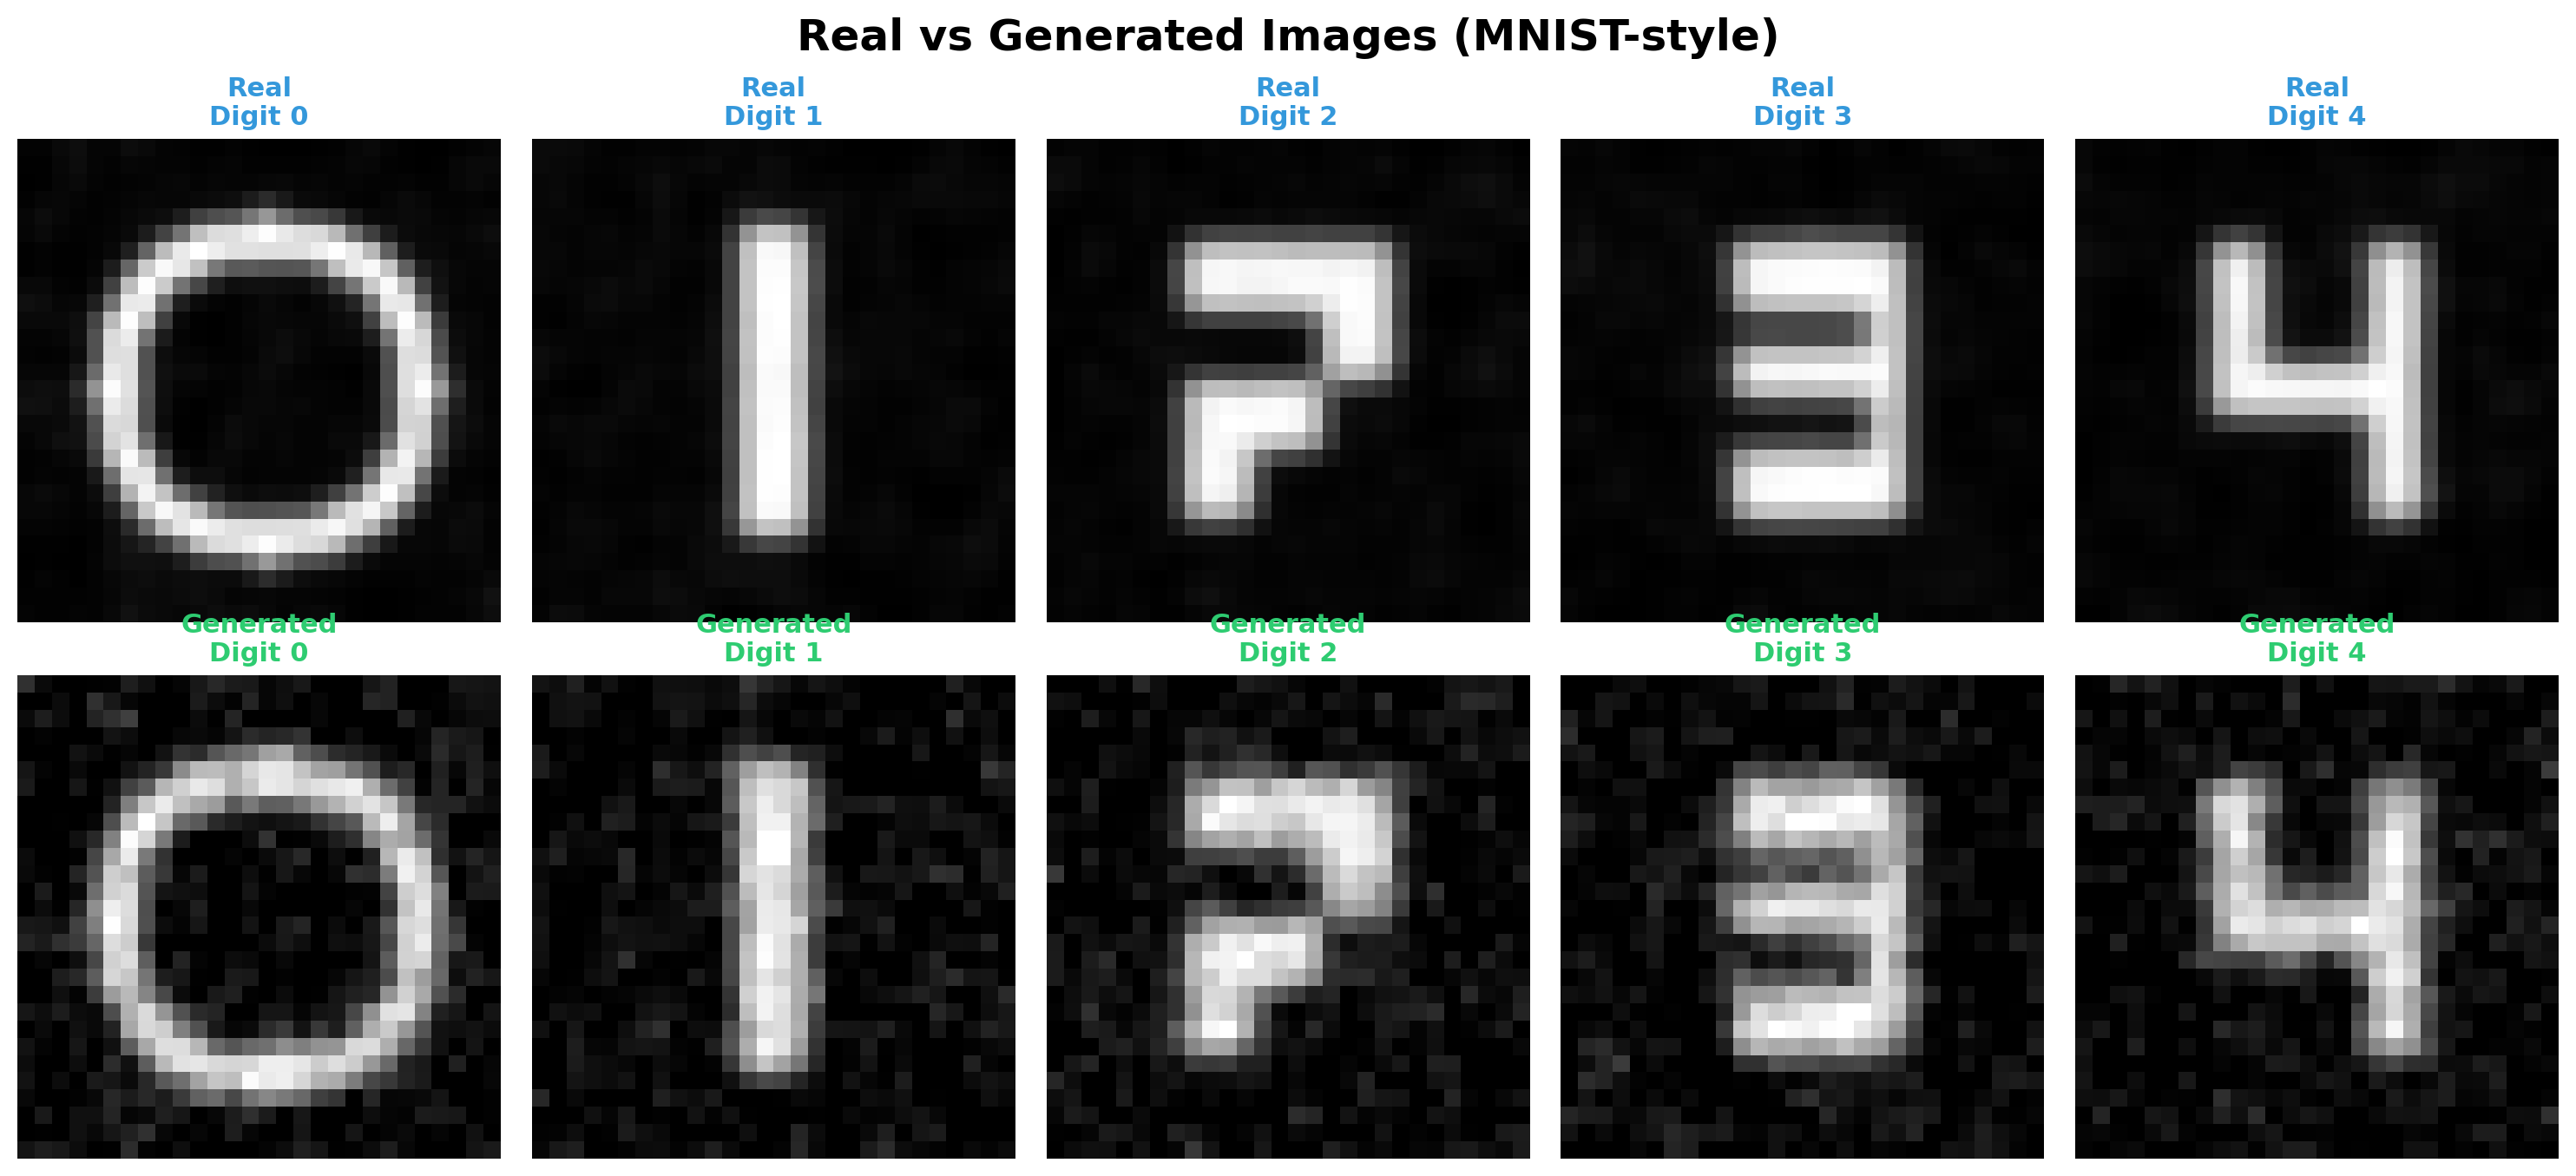
\includegraphics[width=0.75\textwidth]{../figures/generation_examples.png}
\end{center}

Real vs generated MNIST-style digits
\end{frame}

\begin{frame}{Latent Space Interpolation}
\begin{center}
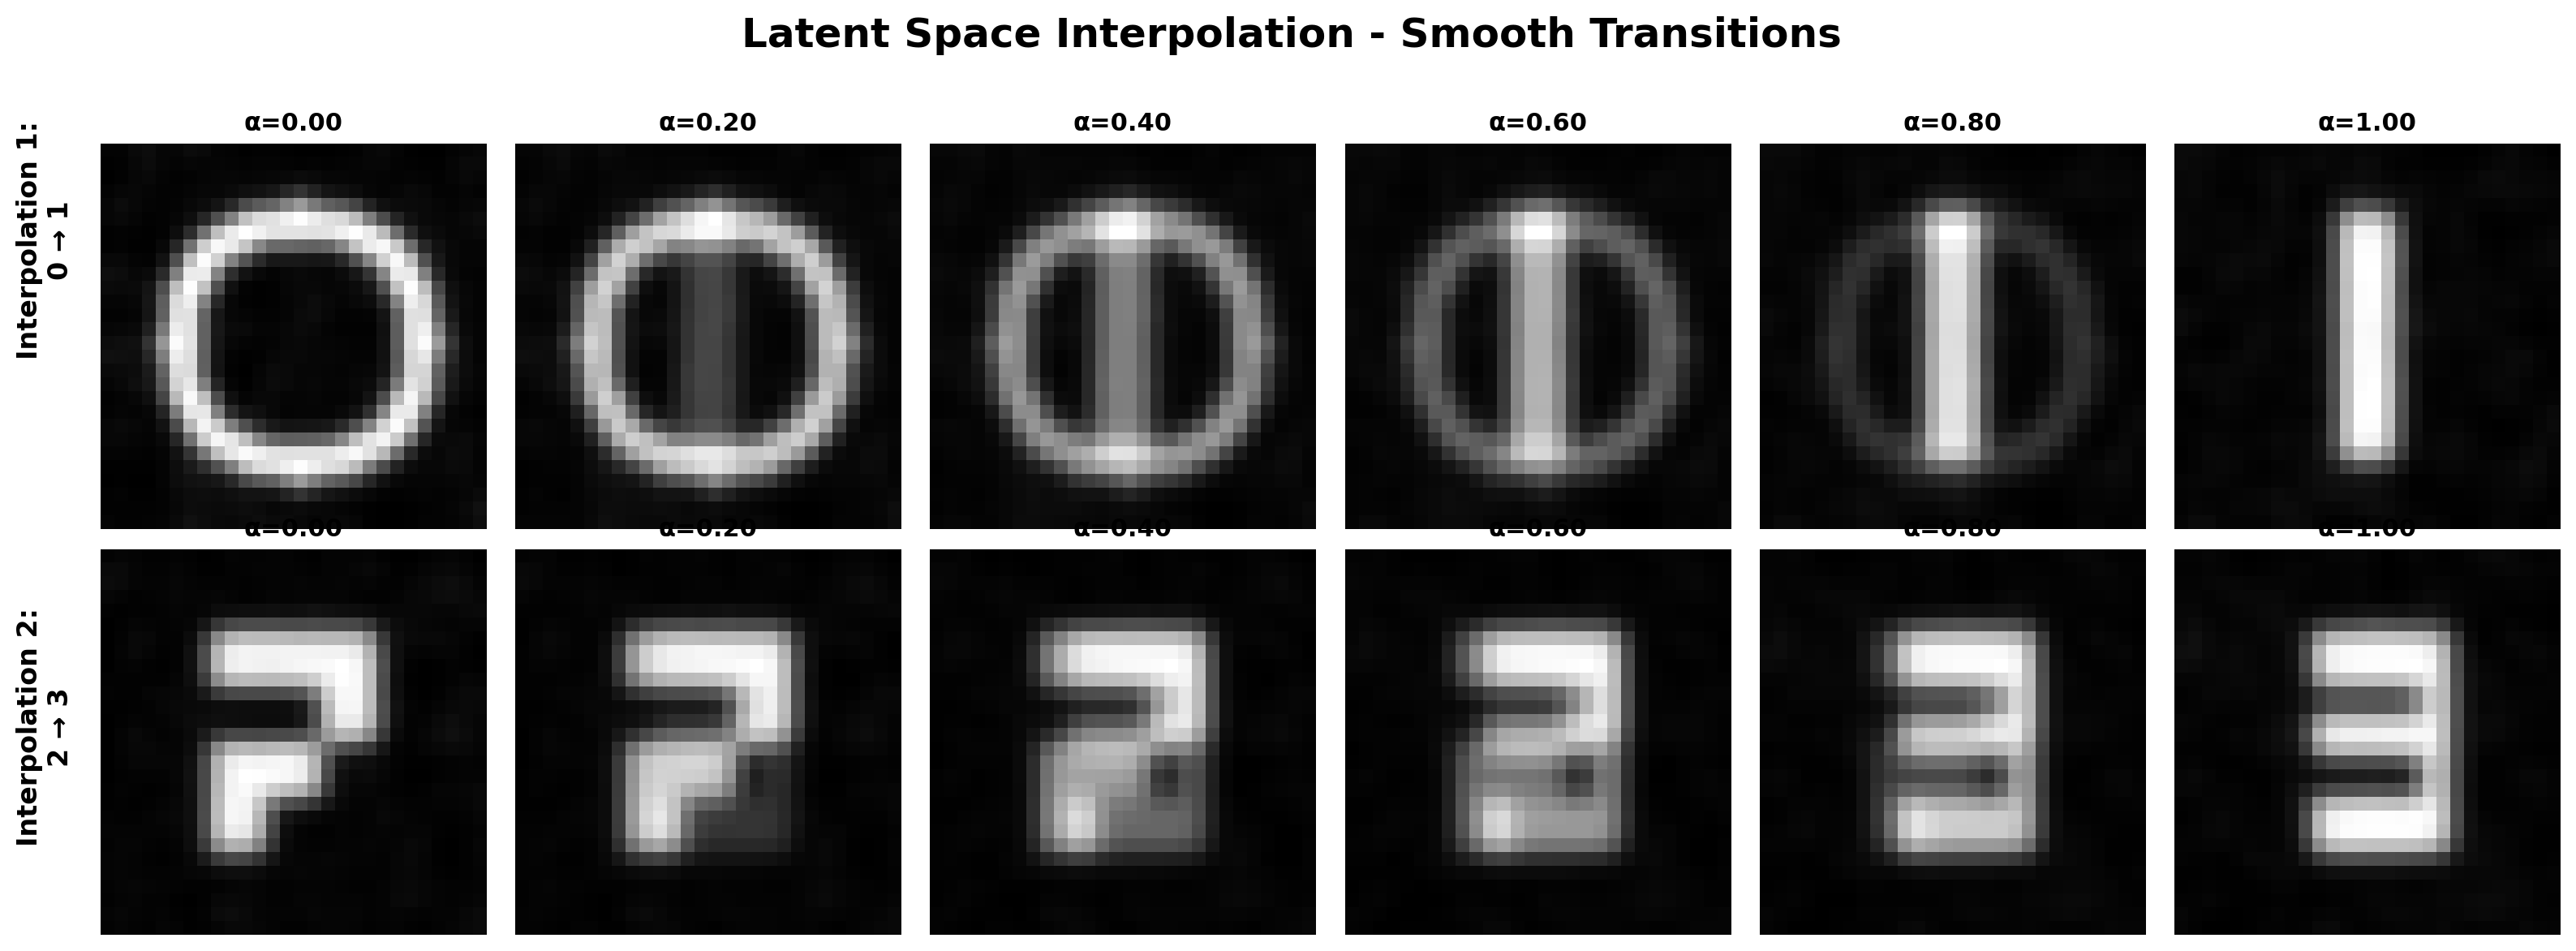
\includegraphics[width=0.85\textwidth]{../figures/latent_interpolation.png}
\end{center}

Smooth transitions between digits in latent space
\end{frame}

\begin{frame}{Conditional Generation}
\begin{center}
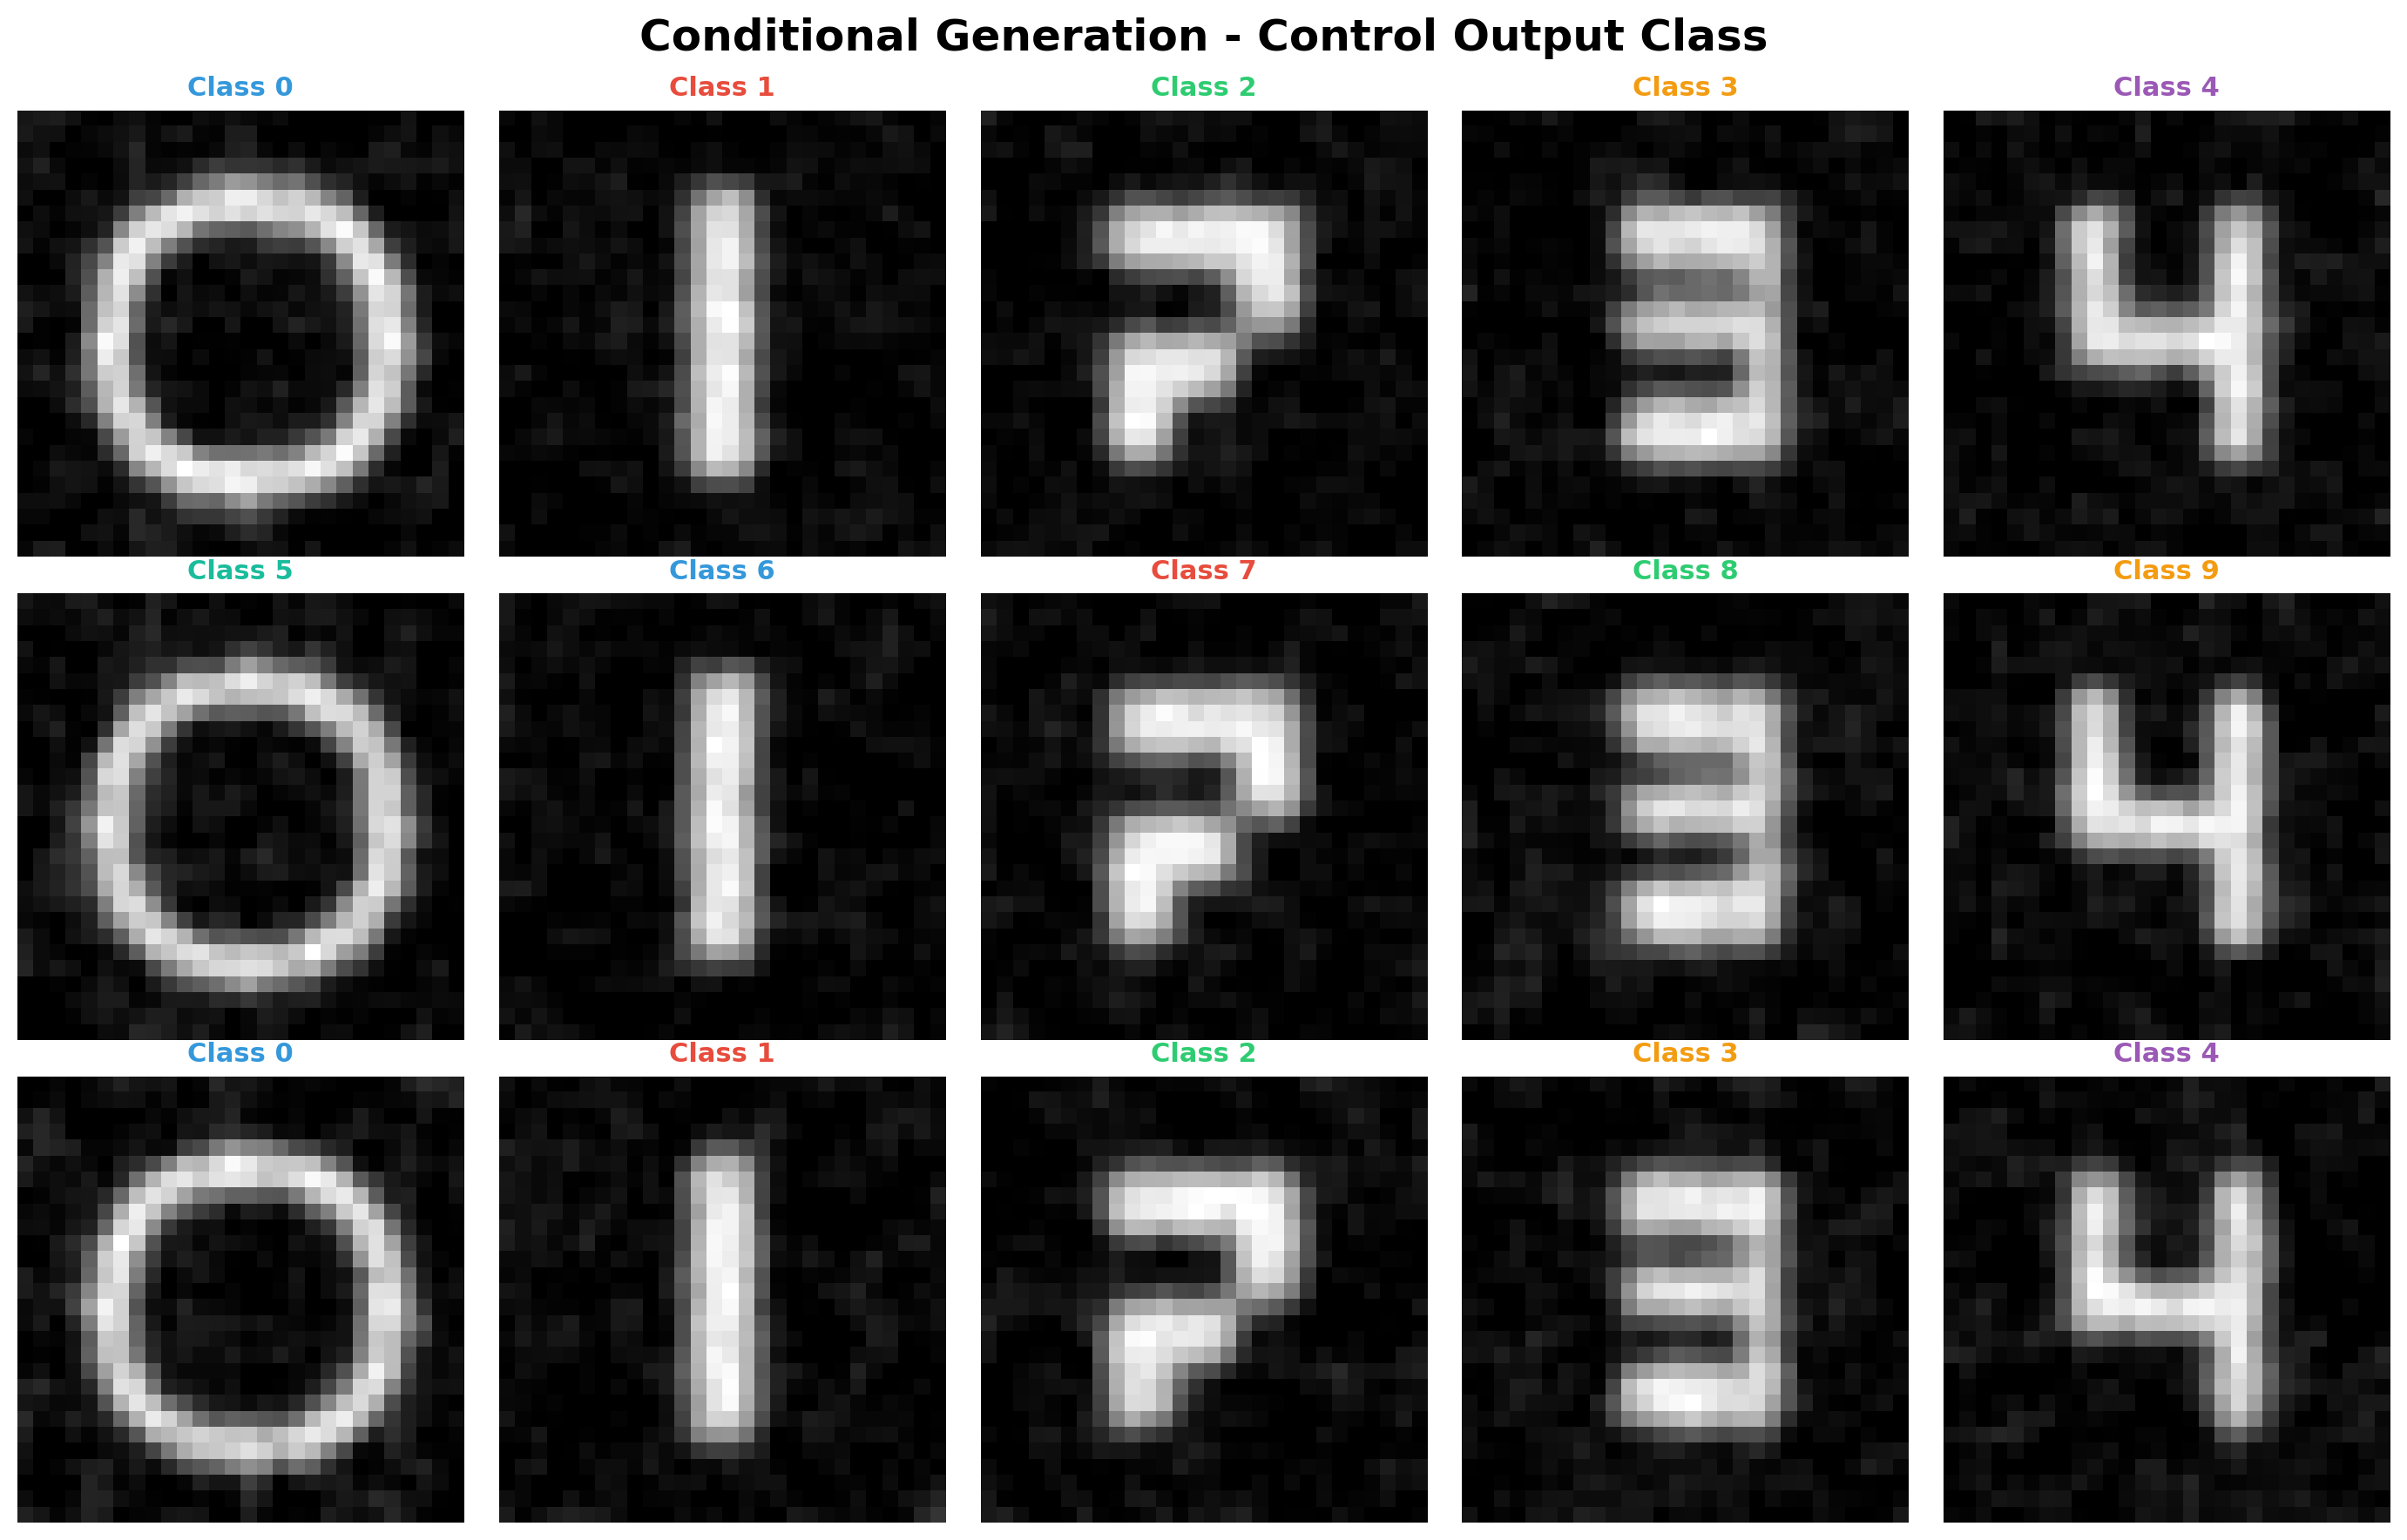
\includegraphics[width=0.65\textwidth]{../figures/conditional_generation.png}
\end{center}

Generate specific classes on demand
\end{frame}

\begin{frame}{Style Transfer}
\begin{center}
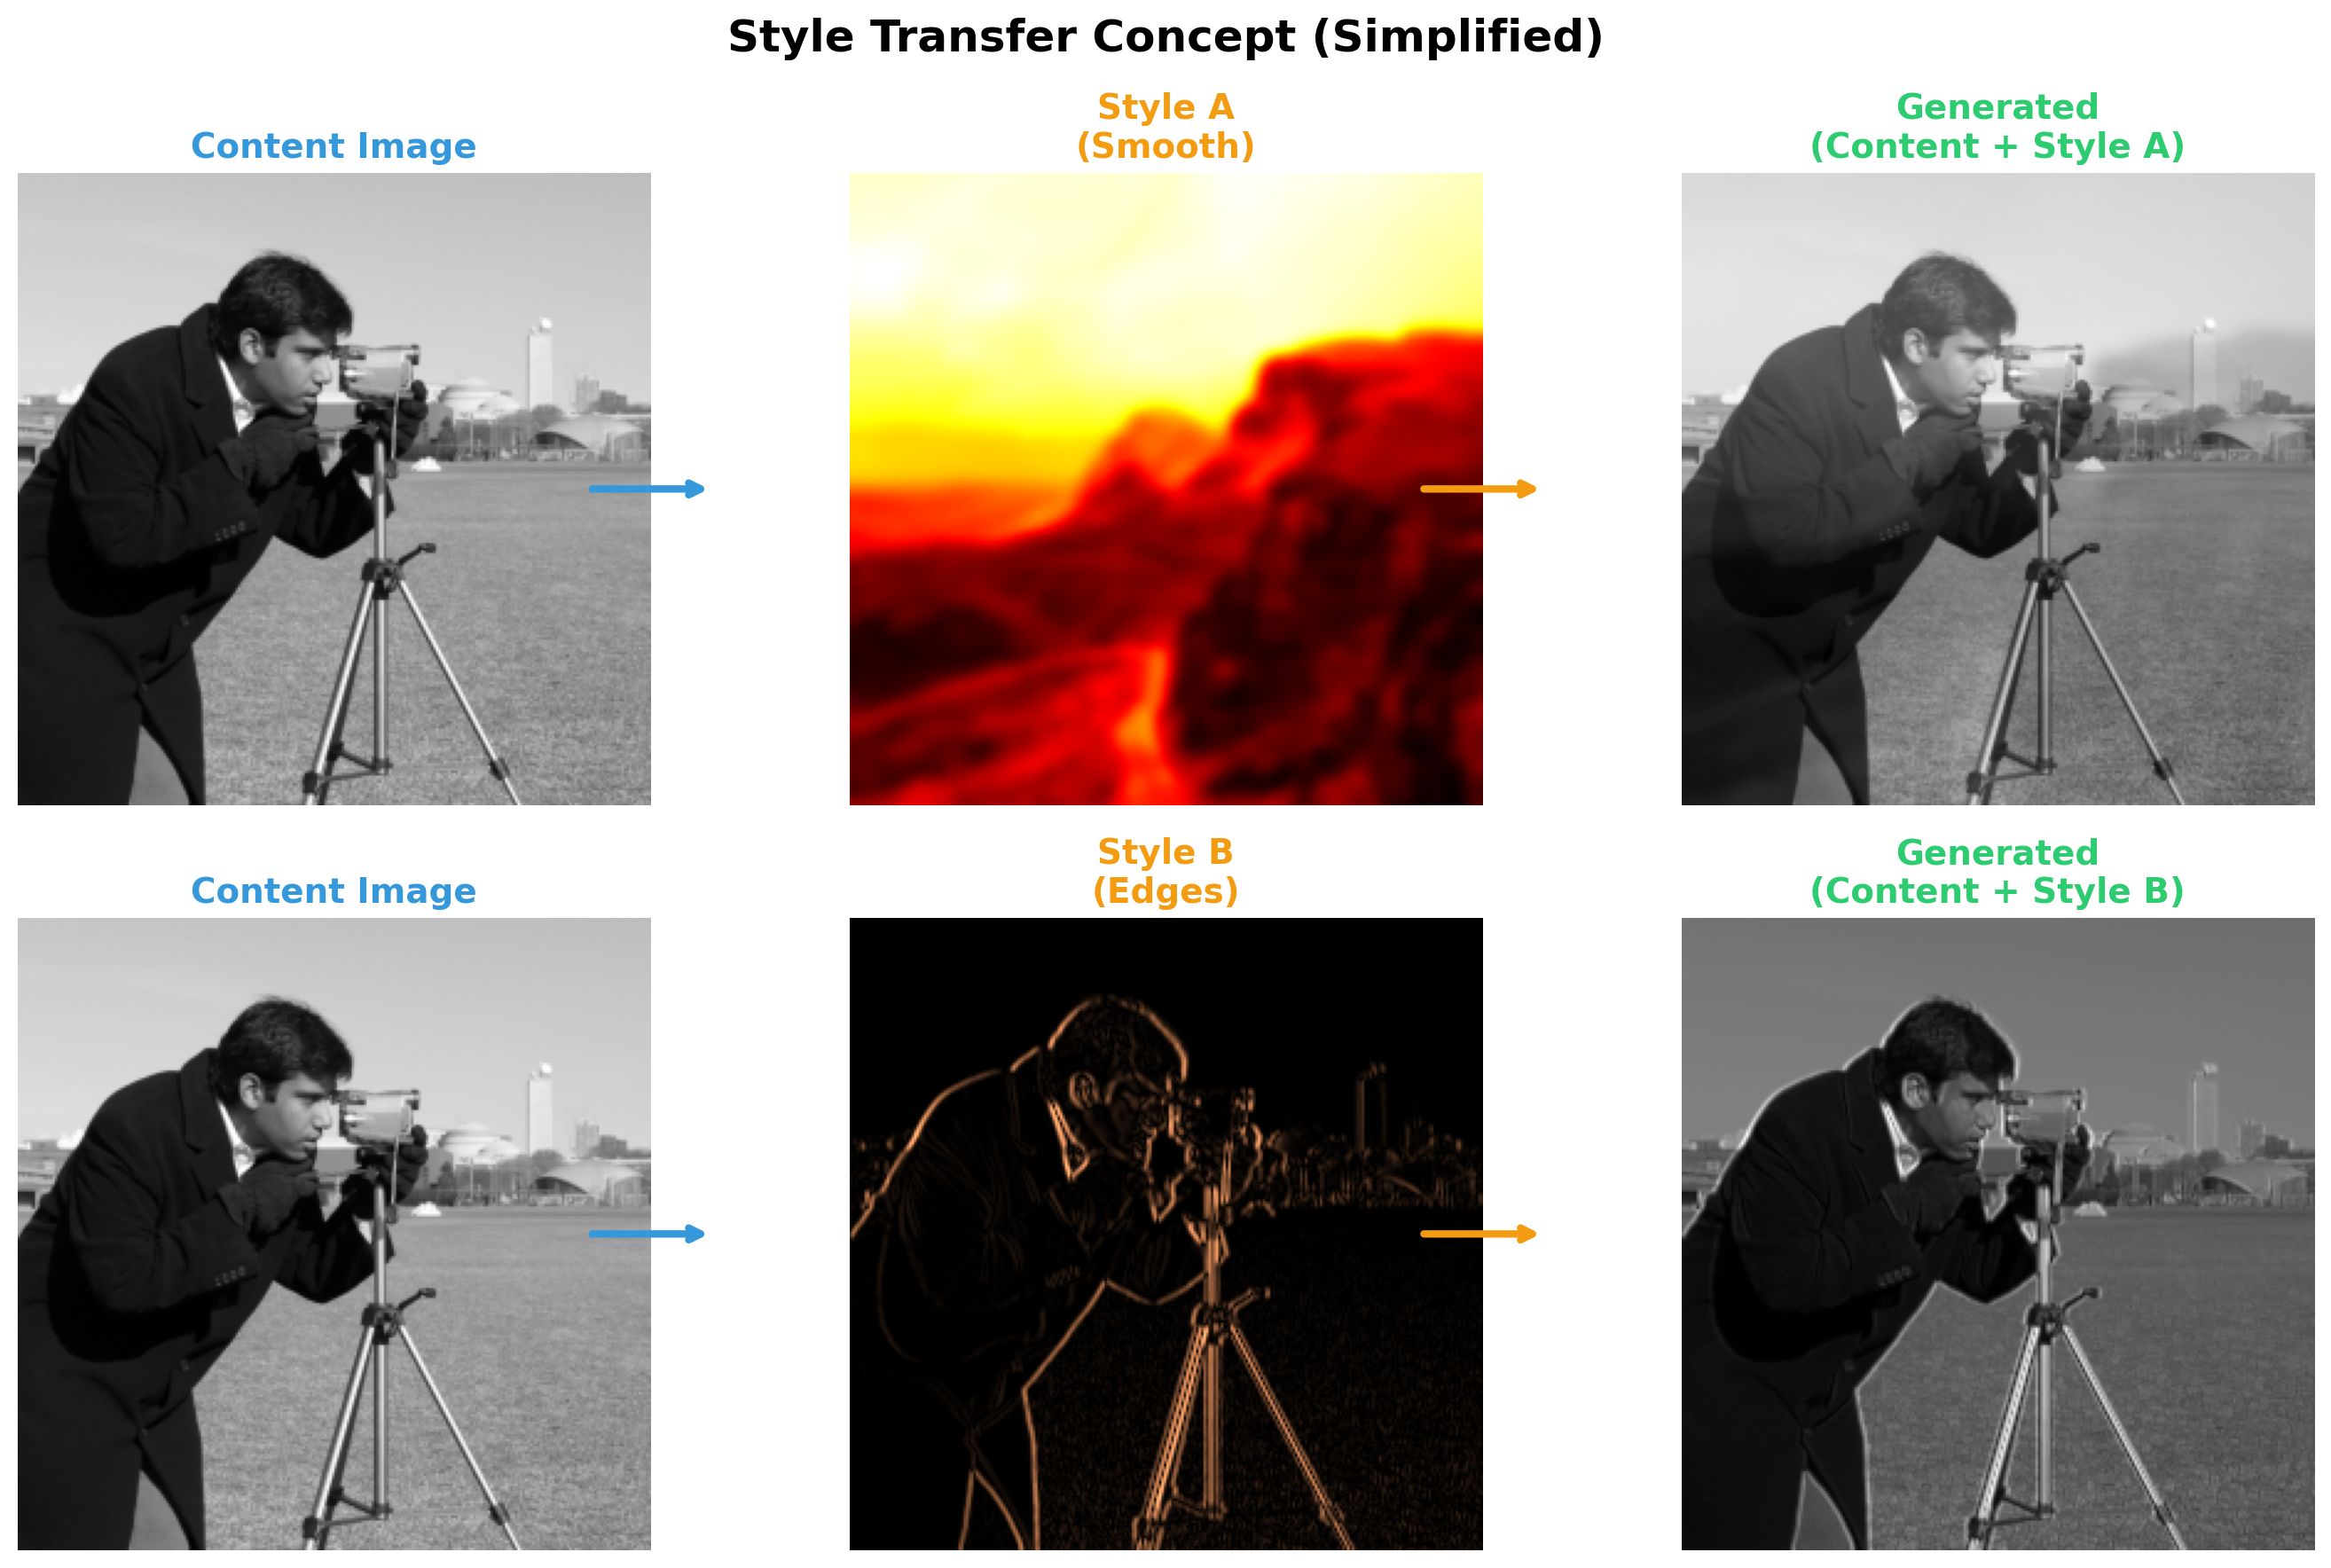
\includegraphics[width=0.6\textwidth]{../figures/style_transfer_concept.png}
\end{center}

Combine content and style
\end{frame}

\begin{frame}{Real-World Applications}
\begin{center}
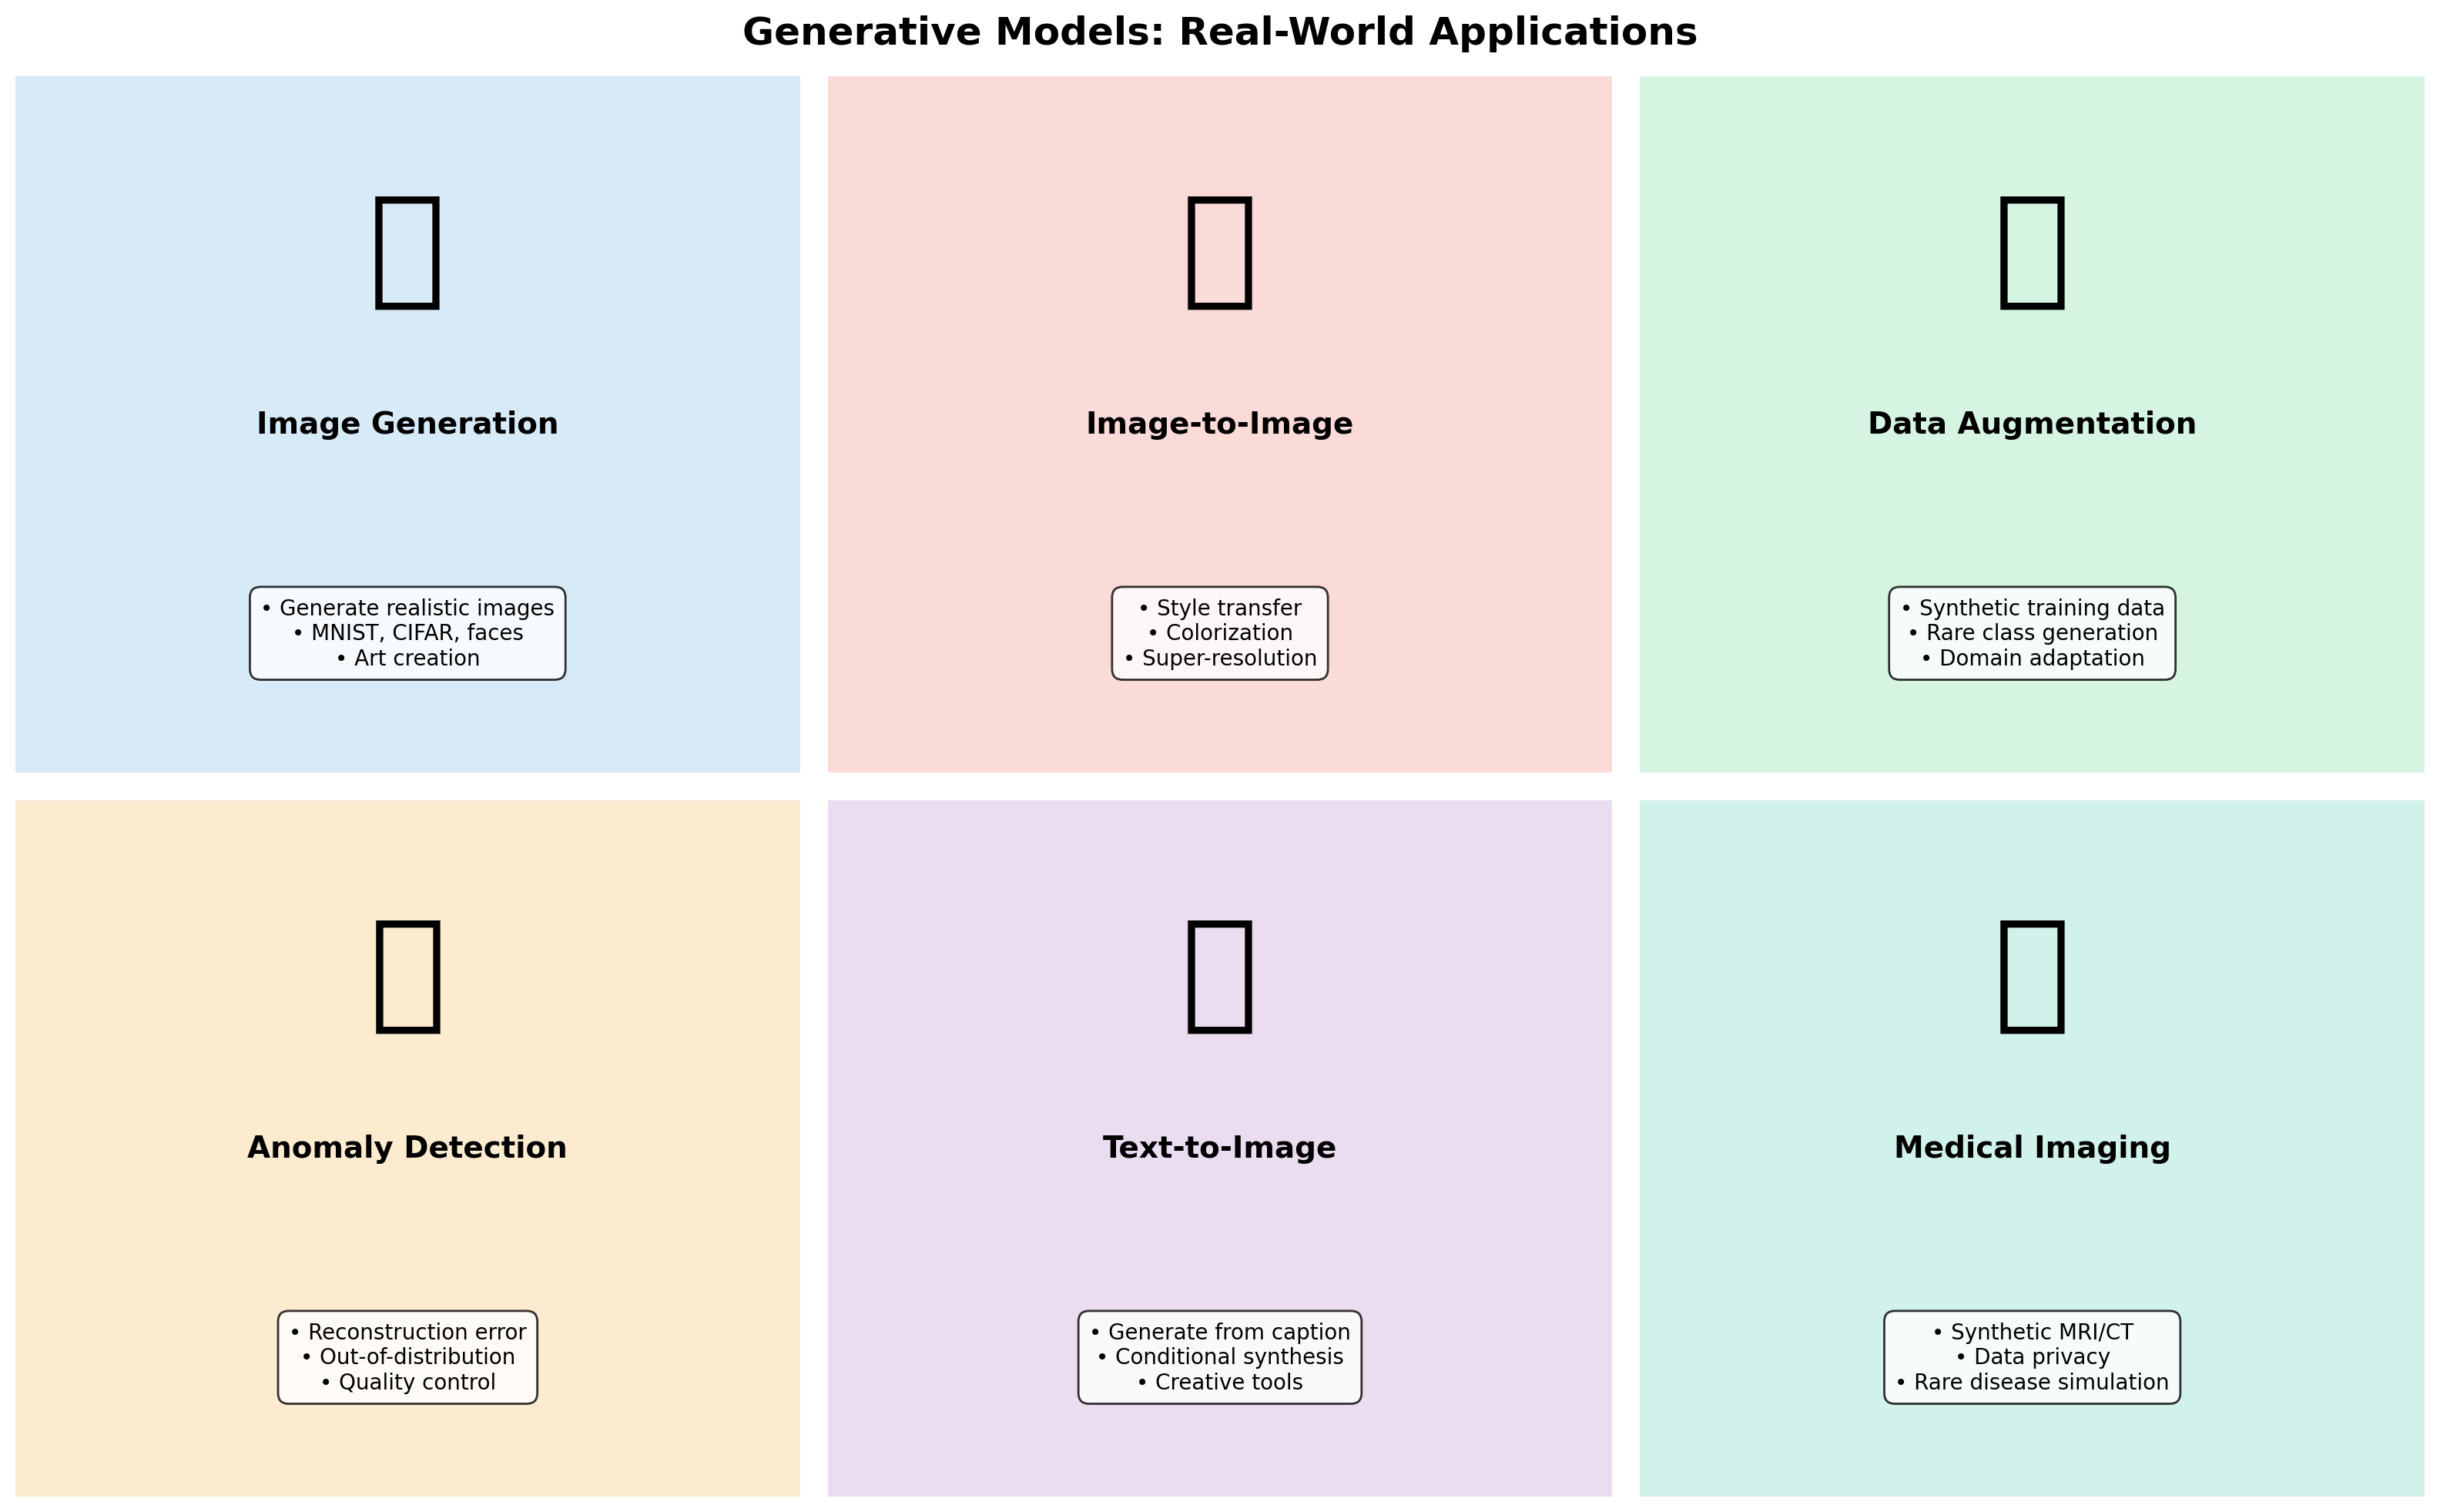
\includegraphics[width=0.7\textwidth]{../figures/applications_overview.png}
\end{center}
\end{frame}

\begin{frame}{Medical Imaging Application}
\textbf{Use Case:} Synthetic medical images for training

\textbf{Benefits:}
\begin{itemize}
\item Privacy: No real patient data needed
\item Augmentation: Generate rare conditions
\item Accessibility: More training data available
\end{itemize}

\textbf{Approach:}
\begin{itemize}
\item Train on real MRI/CT scans
\item Generate synthetic but realistic scans
\item Use for training diagnostic models
\item Validate on real data
\end{itemize}
\end{frame}

\begin{frame}{Data Augmentation}
\textbf{Problem:} Limited training data

\textbf{Solution:} Generate synthetic examples
\begin{itemize}
\item Train generative model on available data
\item Generate new variations
\item Augment training set
\item Improve model performance
\end{itemize}

\textbf{Especially Useful For:}
\begin{itemize}
\item Rare classes
\item Expensive data collection
\item Privacy-sensitive domains
\end{itemize}
\end{frame}

\section{Best Practices}

\begin{frame}{Training Tips and Tricks}
\begin{center}
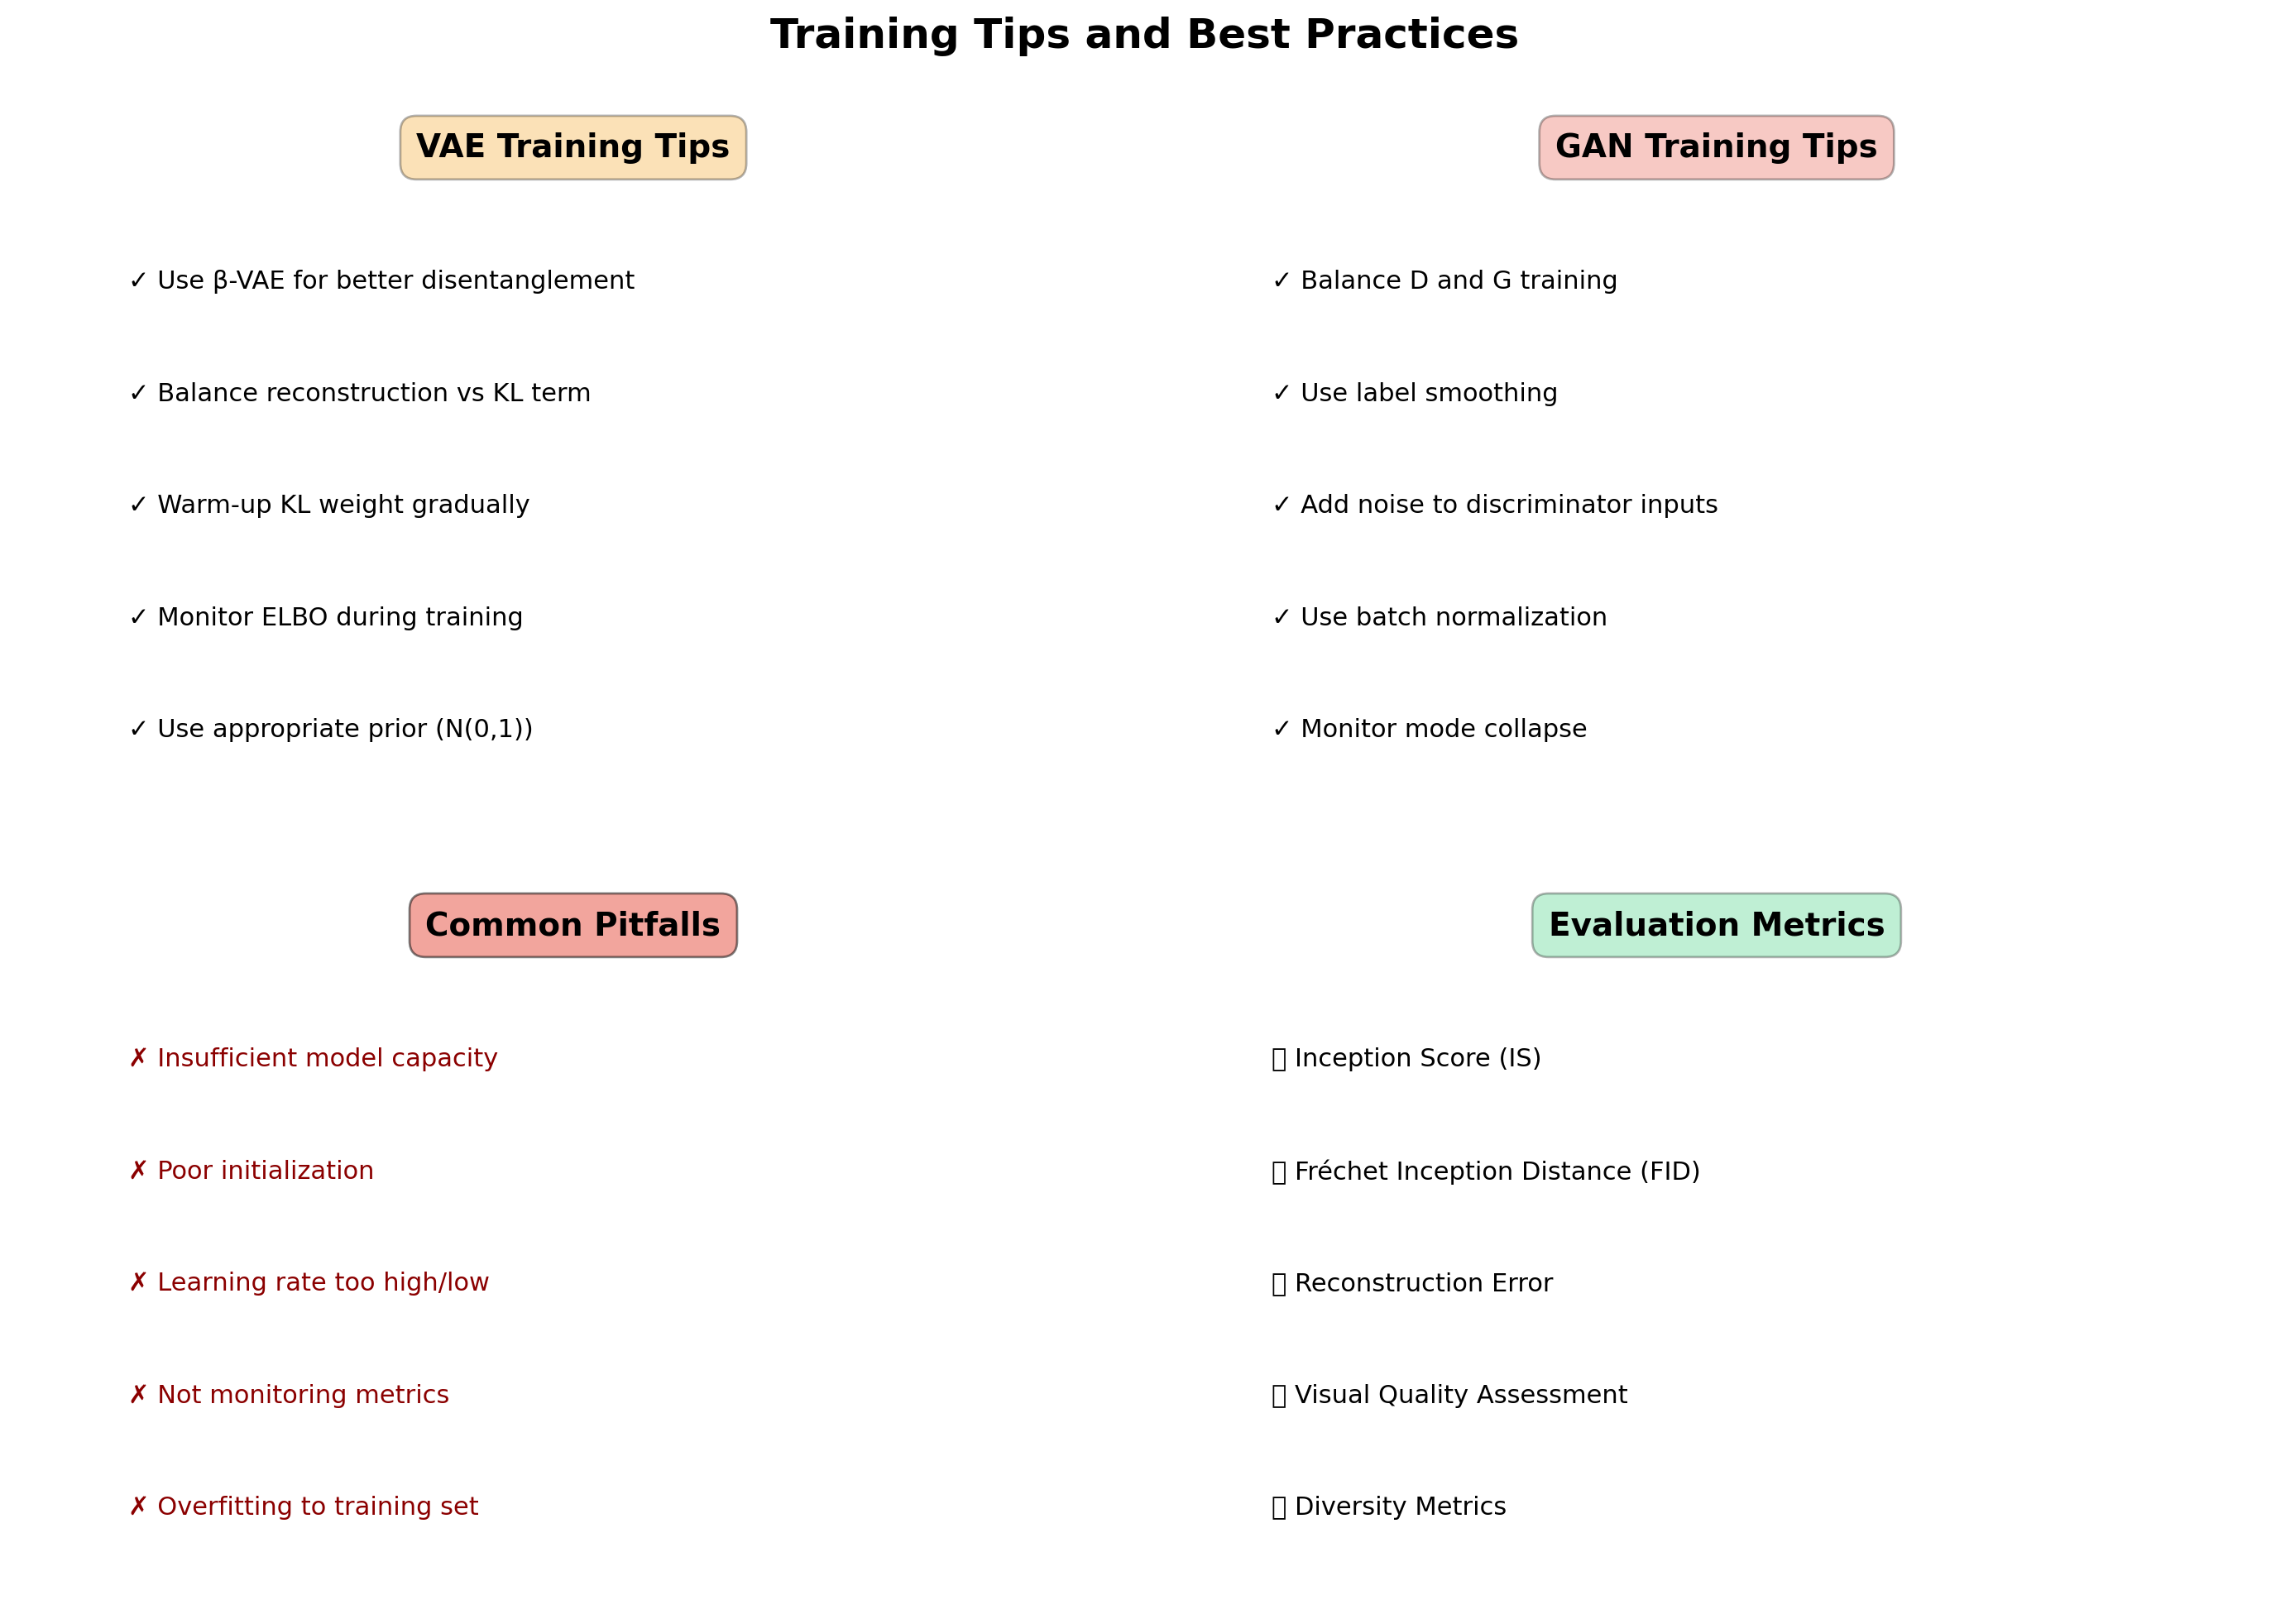
\includegraphics[width=0.65\textwidth]{../figures/training_tips.png}
\end{center}
\end{frame}

\begin{frame}{Debugging Checklist}
\textbf{If VAE produces blurry images:}
\begin{itemize}
\item Reduce KL weight ($\beta$-VAE)
\item Increase latent dimension
\end{itemize}

\textbf{If GAN won't converge:}
\begin{itemize}
\item Balance D and G training
\item Add noise to D inputs
\item Check learning rates (try 0.0002)
\end{itemize}

\textbf{General:}
\begin{itemize}
\item Monitor metrics every epoch
\item Visualize samples frequently
\end{itemize}
\end{frame}

\begin{frame}{Evaluation Metrics}
\textbf{Visual Quality:}
\begin{itemize}
\item Human evaluation (gold standard)
\item Visual inspection of samples
\end{itemize}

\textbf{Quantitative Metrics:}
\begin{itemize}
\item \textbf{Inception Score (IS):} Diversity and quality
\item \textbf{Fréchet Inception Distance (FID):} Distribution similarity
\item \textbf{Reconstruction Error:} For VAE
\end{itemize}

\textbf{Best Practice:} Use multiple metrics, don't rely on one!
\end{frame}

\begin{frame}{Common Pitfalls to Avoid}
\textbf{Don't:}
\begin{itemize}
\item Start with complex architectures
\item Ignore warning signs (mode collapse, divergence)
\item Use only one metric for evaluation
\item Skip hyperparameter tuning
\item Train for too long without checking samples
\end{itemize}

\textbf{Do:}
\begin{itemize}
\item Start simple (MNIST before faces)
\item Monitor training closely
\item Save checkpoints frequently
\item Compare multiple approaches
\item Test on held-out validation set
\end{itemize}
\end{frame}

\section{Summary}

\begin{frame}{Key Takeaways - Part 1}
\textbf{Core Concepts:}
\begin{itemize}
\item Generative models learn to create new data
\item Two main types: VAE and GAN
\item Both learn from examples, generate new samples
\end{itemize}

\textbf{Autoencoders:}
\begin{itemize}
\item Compress and reconstruct
\item Learn useful latent representations
\item Foundation for more complex models
\end{itemize}
\end{frame}

\begin{frame}{Key Takeaways - Part 2}
\textbf{VAE:}
\begin{itemize}
\item Probabilistic framework
\item Smooth latent space
\item Stable but blurry
\end{itemize}

\textbf{GAN:}
\begin{itemize}
\item Adversarial training
\item Sharp realistic outputs
\item Powerful but tricky to train
\end{itemize}
\end{frame}

\begin{frame}{Key Takeaways - Part 3}
\textbf{Applications:}
\begin{itemize}
\item Image generation and manipulation
\item Data augmentation
\item Style transfer
\item Medical imaging
\item Privacy-preserving synthetic data
\end{itemize}

\textbf{Success Factors:}
\begin{itemize}
\item Start simple
\item Monitor carefully
\item Balance stability and quality
\item Use appropriate architecture for task
\end{itemize}
\end{frame}

\begin{frame}{Further Learning}
\textbf{Advanced Topics:}
\begin{itemize}
\item $\beta$-VAE, Conditional GANs
\item StyleGAN, CycleGAN
\item Diffusion Models
\end{itemize}

\textbf{Resources:}
\begin{itemize}
\item Interactive notebook for practice
\item Try MNIST first
\item Experiment with hyperparameters
\end{itemize}
\end{frame}

\begin{frame}[standout]
Questions?
\end{frame}

\end{document}
